\documentclass[11pt,a4paper,oneside]{report}             % Single-side
%\documentclass[11pt,a4paper,twoside,openright]{report}  % Duplex

% thanks to http://tex.stackexchange.com/a/47579/71109
\usepackage{ifxetex}
\usepackage{ifluatex}
\newif\ifxetexorluatex % a new conditional starts as false
\ifnum 0\ifxetex 1\fi\ifluatex 1\fi>0
   \xetexorluatextrue
\fi

\ifxetexorluatex
  \usepackage{fontspec}
\else
  \usepackage[T1]{fontenc}
  \usepackage[utf8]{inputenc}
  \usepackage[lighttt]{lmodern}
  \ttfamily\DeclareFontShape{T1}{lmtt}{m}{it}{<->sub*lmtt/m/sl}{}
\fi

\usepackage[english,magyar]{babel} % Alapértelmezés szerint utoljára definiált nyelv lesz aktív, de később külön beállítjuk az aktív nyelvet.

\usepackage{emptypage} % omit page number on empty pages

%\usepackage{cmap}
\usepackage{amsfonts,amsmath,amssymb} % Mathematical symbols.
%\usepackage[ruled,boxed,resetcount,linesnumbered]{algorithm2e} % For pseudocodes. % beware: this is not compatible with LuaLaTeX, see http://tex.stackexchange.com/questions/34814/lualatex-and-algorithm2e
\usepackage{booktabs} % For publication quality tables for LaTeX
\usepackage{graphicx}

%\usepackage{fancyhdr}
%\usepackage{lastpage}

\usepackage{geometry}
%\usepackage{sectsty}
\usepackage{setspace} % For setting line spacing

\usepackage[unicode]{hyperref} % For hyperlinks in the generated document.
\usepackage{xcolor}
\usepackage{listings} % For source code snippets.

\usepackage[amsmath,thmmarks]{ntheorem} % Theorem-like environments.

\usepackage[hang]{caption}

\singlespacing

\newcommand{\selecthungarian}{
	\selectlanguage{magyar}
	\setlength{\parindent}{2em}
	\setlength{\parskip}{0em}
	\frenchspacing
}

\newcommand{\selectenglish}{
	\selectlanguage{english}
	\setlength{\parindent}{0em}
	\setlength{\parskip}{0.5em}
	\nonfrenchspacing
	\renewcommand{\figureautorefname}{Figure}
	\renewcommand{\tableautorefname}{Table}
	\renewcommand{\partautorefname}{Part}
	\renewcommand{\chapterautorefname}{Chapter}
	\renewcommand{\sectionautorefname}{Section}
	\renewcommand{\subsectionautorefname}{Section}
	\renewcommand{\subsubsectionautorefname}{Section}
}

\usepackage[numbers]{natbib}
\usepackage{xspace}

% https://github.com/GothenburgBitFactory/guides/blob/master/20151107_de_openrheinruhr/yaml_syntax_highlighting.tex

\newcommand\YAMLcolonstyle{\color{red}\mdseries}
\newcommand\YAMLkeystyle{\color{black}\bfseries}
\newcommand\YAMLvaluestyle{\color{blue}\mdseries}

\makeatletter

% here is a macro expanding to the name of the language
% (handy if you decide to change it further down the road)
\newcommand\language@yaml{yaml}

\expandafter\expandafter\expandafter\lstdefinelanguage
\expandafter{\language@yaml}
{
  keywords={true,false,null,y,n},
  keywordstyle=\color{darkgray}\bfseries,
  basicstyle=\YAMLkeystyle,                                 % assuming a key comes first
  sensitive=false,
  comment=[l]{\#},
%  morecomment=[s]{/*}{*/},
  commentstyle=\color{purple}\ttfamily,
  stringstyle=\YAMLvaluestyle\ttfamily,
  moredelim=[l][\color{orange}]{\&},
  moredelim=[l][\color{magenta}]{*},
  moredelim=**[il][\YAMLcolonstyle{:}\YAMLvaluestyle]{:},   % switch to value style at :
  morestring=[b]',
  morestring=[b]",
  literate =    {---}{{\ProcessThreeDashes}}3
                {>}{{\textcolor{red}\textgreater}}1
                {|}{{\textcolor{red}\textbar}}1
                {\ -\ }{{\mdseries\ -\ }}3,
}

% switch to key style at EOL
\lst@AddToHook{EveryLine}{\ifx\lst@language\language@yaml\YAMLkeystyle\fi}
\makeatother

\newcommand\ProcessThreeDashes{\llap{\color{cyan}\mdseries-{-}-}}



\newcommand{\vikszerzoVezeteknev}{Kozák}
\newcommand{\vikszerzoKeresztnev}{Miklós}

\newcommand{\vikkonzulensAMegszolitas}{Dr.~}
\newcommand{\vikkonzulensAVezeteknev}{Zsóka}
\newcommand{\vikkonzulensAKeresztnev}{Zoltán}

\newcommand{\vikkonzulensBMegszolitas}{}
\newcommand{\vikkonzulensBVezeteknev}{}
\newcommand{\vikkonzulensBKeresztnev}{}

\newcommand{\vikkonzulensCMegszolitas}{}
\newcommand{\vikkonzulensCVezeteknev}{}
\newcommand{\vikkonzulensCKeresztnev}{}

\newcommand{\vikcim}{Automated monitoring of IT systems and network devices} % Cím
\newcommand{\viktanszek}{\bmehit} % Tanszék
\newcommand{\vikdoktipus}{\bsc} % Dokumentum típusa (\bsc vagy \msc)
\newcommand{\vikmunkatipusat}{szakdolgozatot} % a "hallgató nyilatkozat" részhez: szakdolgozatot vagy diplomatervet

\newcommand{\szerzoMeta}{\vikszerzoVezeteknev{} \vikszerzoKeresztnev} % egy szerző esetén

%\newcommand{\kszk}{\mbox{KSZK}~}
\newcommand{\kszk}{\mbox{CESIG}~}
%\newcommand{\kszkfull}{Kollégiumi Számítástechnikai Kör~}
\newcommand{\kszkfull}{Computer Engineering Special Interest Group~}
\newcommand{\sch}{dormitory~}
\newcommand{\schfull}{Schönherz Zoltán Dormitory~}

% Settings for English documents
%--------------------------------------------------------------------------------------
% Elnevezések
%--------------------------------------------------------------------------------------
\newcommand{\bme}{Budapest University of Technology and Economics}
\newcommand{\vik}{Faculty of Electrical Engineering and Informatics}

\newcommand{\bmemit}{Department of Measurement and Information Systems}
\newcommand{\bmehit}{Department of Networked Systems and Services}

\newcommand{\keszitette}{Author}
\newcommand{\konzulens}{Advisor}

\newcommand{\bsc}{Bachelor's Thesis}
\newcommand{\msc}{Master's Thesis}
\newcommand{\tdk}{Scientific Students' Association Report}
\newcommand{\bsconlab}{BSc Project Laboratory}
\newcommand{\msconlabi}{MSc Project Laboratory 1}
\newcommand{\msconlabii}{MSc Project Laboratory 2}

\newcommand{\pelda}{Example}
\newcommand{\definicio}{Definition}
\newcommand{\tetel}{Theorem}

\newcommand{\bevezetes}{Introduction}
\newcommand{\koszonetnyilvanitas}{Acknowledgements}
\newcommand{\fuggelek}{Appendix}

% Optional custom titles
%\addto\captionsenglish{%
%\renewcommand*{\listfigurename}{Your list of figures title}
%\renewcommand*{\listtablename}{Your list of tables title}
%\renewcommand*{\bibname}{Your bibliography title}
%}

\newcommand{\szerzo}{\vikszerzoKeresztnev{} \vikszerzoVezeteknev}
\newcommand{\vikkonzulensA}{\vikkonzulensAMegszolitas\vikkonzulensAKeresztnev{} \vikkonzulensAVezeteknev}
\newcommand{\vikkonzulensB}{\vikkonzulensBMegszolitas\vikkonzulensBKeresztnev{} \vikkonzulensBVezeteknev}
\newcommand{\vikkonzulensC}{\vikkonzulensCMegszolitas\vikkonzulensCKeresztnev{} \vikkonzulensCVezeteknev}

\newcommand{\selectthesislanguage}{\selectenglish}

\bibliographystyle{plainnat}

\newcommand{\ie}{i.e.\@\xspace}
\newcommand{\Ie}{I.e.\@\xspace}
\newcommand{\eg}{e.g.\@\xspace}
\newcommand{\Eg}{E.g.\@\xspace}
\newcommand{\etal}{et al.\@\xspace}
\newcommand{\etc}{etc.\@\xspace}
\newcommand{\vs}{vs.\@\xspace}
\newcommand{\viz}{viz.\@\xspace} % videlicet
\newcommand{\cf}{cf.\@\xspace} % confer
\newcommand{\Cf}{Cf.\@\xspace}
\newcommand{\wrt}{w.r.t.\@\xspace} % with respect to
\newcommand{\approximately}{approx.\@\xspace}

\newcommand{\appendixnumber}{1}  % a fofejezet-szamlalo az angol ABC 1. betuje (A) lesz


%--------------------------------------------------------------------------------------
% Page layout setup
%--------------------------------------------------------------------------------------
% we need to redefine the pagestyle plain
% another possibility is to use the body of this command without \fancypagestyle
% and use \pagestyle{fancy} but in that case the special pages
% (like the ToC, the References, and the Chapter pages)remain in plane style

\pagestyle{plain}
\geometry{inner=35mm, outer=25mm, top=28mm, bottom=25mm}

\setcounter{tocdepth}{3}
%\sectionfont{\large\upshape\bfseries}
\setcounter{secnumdepth}{3}

\sloppy % Margón túllógó sorok tiltása.
\widowpenalty=10000 \clubpenalty=10000 %A fattyú- és árvasorok elkerülése
\def\hyph{-\penalty0\hskip0pt\relax} % Kötőjeles szavak elválasztásának engedélyezése


%--------------------------------------------------------------------------------------
% Setup hyperref package
%--------------------------------------------------------------------------------------
\hypersetup{
    % bookmarks=true,            % show bookmarks bar?
    unicode=true,              % non-Latin characters in Acrobat's bookmarks
    pdftitle={\vikcim},        % title
    pdfauthor={\szerzoMeta},    % author
    pdfsubject={\vikdoktipus}, % subject of the document
    pdfcreator={\szerzoMeta},   % creator of the document
    pdfproducer={},    % producer of the document
    pdfkeywords={},    % list of keywords (separate then by comma)
    pdfnewwindow=true,         % links in new window
    colorlinks=true,           % false: boxed links; true: colored links
    linkcolor=black,           % color of internal links
    citecolor=black,           % color of links to bibliography
    filecolor=black,           % color of file links
    urlcolor=black             % color of external links
}


%--------------------------------------------------------------------------------------
% Set up listings
%--------------------------------------------------------------------------------------
\definecolor{lightgray}{rgb}{0.95,0.95,0.95}
\lstset{
	basicstyle=\scriptsize\ttfamily, % print whole listing small
	keywordstyle=\color{black}\bfseries, % bold black keywords
	identifierstyle=, % nothing happens
	% default behavior: comments in italic, to change use
	% commentstyle=\color{green}, % for e.g. green comments
	stringstyle=\scriptsize,
	showstringspaces=false, % no special string spaces
	aboveskip=3pt,
	belowskip=3pt,
	backgroundcolor=\color{lightgray},
	columns=flexible,
	keepspaces=true,
	escapeinside={(*@}{@*)},
	captionpos=b,
	breaklines=true,
	frame=single,
	float=!ht,
	tabsize=2,
	literate=*
		{á}{{\'a}}1	{é}{{\'e}}1	{í}{{\'i}}1	{ó}{{\'o}}1	{ö}{{\"o}}1	{ő}{{\H{o}}}1	{ú}{{\'u}}1	{ü}{{\"u}}1	{ű}{{\H{u}}}1
		{Á}{{\'A}}1	{É}{{\'E}}1	{Í}{{\'I}}1	{Ó}{{\'O}}1	{Ö}{{\"O}}1	{Ő}{{\H{O}}}1	{Ú}{{\'U}}1	{Ü}{{\"U}}1	{Ű}{{\H{U}}}1
}


%--------------------------------------------------------------------------------------
% Set up theorem-like environments
%--------------------------------------------------------------------------------------
% Using ntheorem package -- see http://www.math.washington.edu/tex-archive/macros/latex/contrib/ntheorem/ntheorem.pdf

\theoremstyle{plain}
\theoremseparator{.}
\newtheorem{example}{\pelda}

\theoremseparator{.}
%\theoremprework{\bigskip\hrule\medskip}
%\theorempostwork{\hrule\bigskip}
\theorembodyfont{\upshape}
\theoremsymbol{{\large \ensuremath{\centerdot}}}
\newtheorem{definition}{\definicio}

\theoremseparator{.}
%\theoremprework{\bigskip\hrule\medskip}
%\theorempostwork{\hrule\bigskip}
\newtheorem{theorem}{\tetel}


%--------------------------------------------------------------------------------------
% Some new commands and declarations
%--------------------------------------------------------------------------------------
\newcommand{\code}[1]{{\upshape\ttfamily\scriptsize\indent #1}}
\newcommand{\doi}[1]{DOI: \href{http://dx.doi.org/\detokenize{#1}}{\raggedright{\texttt{\detokenize{#1}}}}} % A hivatkozások közt így könnyebb DOI-t megadni.

\DeclareMathOperator*{\argmax}{arg\,max}
%\DeclareMathOperator*[1]{\floor}{arg\,max}
\DeclareMathOperator{\sign}{sgn}
\DeclareMathOperator{\rot}{rot}


%--------------------------------------------------------------------------------------
% Setup captions
%--------------------------------------------------------------------------------------
\captionsetup[figure]{aboveskip=10pt}

\renewcommand{\captionlabelfont}{\bf}
%\renewcommand{\captionfont}{\footnotesize\it}

%--------------------------------------------------------------------------------------
% Hyphenation exceptions
%--------------------------------------------------------------------------------------
\hyphenation{Shakes-peare Mar-seilles ár-víz-tű-rő tü-kör-fú-ró-gép}


\author{\vikszerzo}
\title{\viktitle}


%--------------------------------------------------------------------------------------
% Table of contents and the main text
%--------------------------------------------------------------------------------------
\begin{document}

\pagenumbering{gobble}

\selectthesislanguage

% Titlepage -- choose one from below
%~~~~~~~~~~~~~~~~~~~~~~~~~~~~~~~~~~~~~~~~~~~~~~~~~~~~~~~~~~~~~~~~~~~~~~~~~~~~~~~~~~~~~~
\hypersetup{pageanchor=false}
%--------------------------------------------------------------------------------------
%	The title page
%--------------------------------------------------------------------------------------
\begin{titlepage}
\begin{center}

\includegraphics[width=60mm,keepaspectratio]{figures/bme_logo.pdf}\\
\vspace{0.3cm}
\textbf{\bme}\\
\textmd{\vik}\\
\textmd{\viktanszek}\\[5cm]

\vspace{0.4cm}
{\huge \bfseries \vikcim}\\[0.8cm]
\vspace{0.5cm}
\textsc{\Large \vikdoktipus}\\[4cm]

{
	\renewcommand{\arraystretch}{0.85}
	\begin{tabular}{cc}
	 \makebox[7cm]{\emph{\keszitette}} & \makebox[7cm]{\emph{\konzulens}} \\ \noalign{\smallskip}
	 \makebox[7cm]{\szerzo} & \makebox[7cm]{\vikkonzulensA} \\
	  & \makebox[7cm]{\vikkonzulensB} \\
	  & \makebox[7cm]{\vikkonzulensC} \\
	\end{tabular}
}

\vfill
{\large \today}
\end{center}
\end{titlepage}
\hypersetup{pageanchor=false}

		   % Szakdolgozat/Diplomaterv címlap


% Table of Contents
%~~~~~~~~~~~~~~~~~~~~~~~~~~~~~~~~~~~~~~~~~~~~~~~~~~~~~~~~~~~~~~~~~~~~~~~~~~~~~~~~~~~~~~
\tableofcontents\cleardoublepage


% Declaration and Abstract
%~~~~~~~~~~~~~~~~~~~~~~~~~~~~~~~~~~~~~~~~~~~~~~~~~~~~~~~~~~~~~~~~~~~~~~~~~~~~~~~~~~~~~~
\selectlanguage{magyar}
\pagenumbering{gobble}
%--------------------------------------------------------------------------------------
% Nyilatkozat
%--------------------------------------------------------------------------------------
\begin{center}
\large
\textbf{HALLGATÓI NYILATKOZAT}\\
\end{center}

Alulírott \emph{\vikszerzoVezeteknev{} \vikszerzoKeresztnev}, szigorló hallgató kijelentem, hogy ezt a \vikmunkatipusat{} meg nem engedett segítség nélkül, saját magam készítettem, csak a megadott forrásokat (szakirodalom, eszközök stb.) használtam fel. Minden olyan részt, melyet szó szerint, vagy azonos értelemben, de átfogalmazva más forrásból átvettem, egyértelműen, a forrás megadásával megjelöltem.

Hozzájárulok, hogy a jelen munkám alapadatait (szerző(k), cím, angol és magyar nyelvű tartalmi kivonat, készítés éve, konzulens(ek) neve) a BME VIK nyilvánosan hozzáférhető elektronikus formában, a munka teljes szövegét pedig az egyetem belső hálózatán keresztül (vagy autentikált felhasználók számára) közzétegye. Kijelentem, hogy a benyújtott munka és annak elektronikus verziója megegyezik. Dékáni engedéllyel titkosított diplomatervek esetén a dolgozat szövege csak 3 év eltelte után válik hozzáférhetővé.

\begin{flushleft}
\vspace*{1cm}
Budapest, \today
\end{flushleft}

\begin{flushright}
 \vspace*{1cm}
 \makebox[7cm]{\rule{6cm}{.4pt}}\\
 \makebox[7cm]{\emph{\vikszerzoVezeteknev{} \vikszerzoKeresztnev}}\\
 \makebox[7cm]{hallgató}
\end{flushright}
\thispagestyle{empty}

\vfill
\cleardoublepage

\selectthesislanguage
 % Hallgatói nyilatkozat
\pagenumbering{roman}
\setcounter{page}{1}

\selecthungarian

%----------------------------------------------------------------------------
% Abstract in Hungarian
%----------------------------------------------------------------------------
\chapter*{Kivonat}\addcontentsline{toc}{chapter}{Kivonat}

Az automatikus felügyelő rendszerek feladata metrikákat gyűjteni hardverekről
és szolgáltatásokról, hibákat találni és megpróbálni előre megjósolni a jövőben
bekövetkező meghibásodásokat. Amennyiben szükséges értesítik a megfelelő
személyzetet, hogy gyorsan intézkedhessenek ezáltal megakadályozva, hogy a
probléma túl sok felhasználóra legyen hatással. A modern rendszerek támogatják
továbba a naplóbejegyzések gyűjtését és fejlett elemzését, illetve minden
elérhető adat vizualizációját.

A Kollégiumi Számítástechnikai Kör (röviden KSZK) aktív tagsága nagyjából 20
fő. Ők a Villamosmérnöki és Informatikai Kar olyan hallgatói, akik önkéntesként
teszik munkájukat. Ők különféle informatikai szolgáltatásokat üzemeltetnek a
VIK hallgatói számára és emellett a Schönherz Zoltán Kollégium teljes hálózatát
is üzemeltetik.

A szakdolgozatomban egy automatikus felügyelő rendszer megvalósítását mutatom
be. Az elkészült rendszerben VictoriaMetrics gyűjti a metrikákat a szerverekről
és a hálózati eszközökről egyaránt. A VMAlertmanager komponens küldi a
riasztási értesítéseket egy Mattermost szerverre. Loki és Promtail gyűjti be és
dolgozza fel a naplóbejegyzéseket. Folyamatos Integrációt használok új
felügyelési célpontok bekötésére a futó rendszerbe úgy, hogy egy felügyelő
rendszer adminisztrátor közbenjárására sincs szükség.

Ez az új rendszer remélhetőleg segíteni fog a KSZK-nak emelni szolgáltatásai
színvonalát miközben csökkenti a tagjaira hárult terheket.

Ebben a dolgozatban leírom a teljes folyamatot, melynek eredménye a fent leírt
rendszer implementálása. Tanulmányozom a KSZK által korábban megvalósított
rendszereket annak érdekében, hogy rájöjjek mi kell egy sikeres
megvalósításhoz. Ezen eredmények alapján leírom a KSZK-ban futó felügyelő
rendszer kemény követelményeit és felkutatok olyan modern technológiákat,
amelyek ki tudják elégíteni ezen követelményeket. Az így szerzett tudást
felhasználva meghatározom egy VictoriaMetrics alapú rendszer szerkezetét, majd
elkezdem kidolgozni a részleteket és megvalósítani a tervet. Értékelem az új
rendszert és ellenőrzöm az elért eredményeket. Végül kifejtem miket lehetne még
tenni a jövőben, beleértve lehetséges továbbfejlesztéseket és teljesen új
ötleteket is.

A dolgozat során elkészült rendszer megfelel a felállított követelményeknek. A
KSZK tagjai már használatba is vették az elkészült funkciókat és a Folyamatos
Integráció segítségével sok új rendszert kezdtek el megfigyelni.


\vfill
\selectenglish


%----------------------------------------------------------------------------
% Abstract in English
%----------------------------------------------------------------------------
\chapter*{Abstract}\addcontentsline{toc}{chapter}{Abstract}

Automated monitoring systems collect metrics from hardwares and services,
detect error conditions and try to predict future failures. If neccessary the
right personnel are notified to take immediate action preventing the issue from
affecting too many users. Modern systems also support the collection of logs as
well as advanced analysis and visualization of every available data.

\kszkfull (\kszk for short) is a team of around 20 day-to-day active members.
They are volunteers from the students of \vik. They provide various IT services
for the Faculty's students and are responsible for the operation of \schfull's
whole network.

In this thesis I implement an automated monitoring system. VictoriaMetrics
scrapes metrics from servers and network devices. VMAlertmanager sends alert
notifications to a Mattermost server. Loki and Promtail collect and process
logs. Grafana visualizes collected metrics and logs. Continous Integration is
used to integrate new monitoring targets into the running system without the
intervention of a monitoring system administrator.

This new system will hopefully help \kszk improve the quality of their services
while reducing workload on members.

In this thesis I describe the whole process resulting in the implementation of
the system described above. I study earlier takes on implementing such systems
by \kszk to figure out what is needed for a successful implementation. Based on
these results I establish the hard requirements for a monitoring system in
\kszk's infrastructure and explore modern technologies that can satisfy these
requirements. Using the knowledge gained I describe the new system architecture
for a VictoriaMetrics based solution and implement the specified architecture
and work out the details. I evaluate the new system and check out the results.
Finally I future work including possible improvements and new ideas as well.

The implemented system satisfies the requirements established in this thesis.
Members of \kszk are already using the completed functions and started
monitoring various new systems with Continous Integration.


\vfill
\cleardoublepage

\selectthesislanguage

\newcounter{romanPage}
\setcounter{romanPage}{\value{page}}
\stepcounter{romanPage}
    % Összefoglaló


% The main part of the thesis
%~~~~~~~~~~~~~~~~~~~~~~~~~~~~~~~~~~~~~~~~~~~~~~~~~~~~~~~~~~~~~~~~~~~~~~~~~~~~~~~~~~~~~~
\pagenumbering{arabic}

%----------------------------------------------------------------------------
% 0. Probléma ismertetése röviden
%   - Mi az a monitoring & alerting, miért jó nekünk
%
% Bevezetés: a feladat értelmezése, a tervezés célja, a feladat indokoltsága, a
% diplomaterv felépítésének rövid összefoglalása
%
% A bevezető tartalmazza a diplomaterv-kiírás elemzését, történelmi
% előzményeit, a feladat indokoltságát (a motiváció leírását), az eddigi
% megoldásokat, és ennek tükrében a hallgató megoldásának összefoglalását.
%
% A bevezető szokás szerint a diplomaterv felépítésével záródik, azaz annak
% rövid leírásával, hogy melyik fejezet mivel foglalkozik.

\chapter{Introduction \label{ch0}}
%\chapter{Earlier monitoring systems implemented in the dormitory}
%\chapter{Requirements of the new monitoring system}
%\chapter{Available industry standard technologies}
%\chapter{System architecture}
%\chapter{Implementation details and experiences}
%\chapter{Results and evaluation}
%\chapter{Future development opportunities}
%----------------------------------------------------------------------------

%----------------------------------------------------------------------------
\section{Monitoring Systems}
%----------------------------------------------------------------------------

Maintaining one or two servers for personal purposes is not a daunting task. We
can easily keep an eye on our hardwares and apply fixes when necessary. And if
for some reason a server goes down it is not likely to cause issues for others.

In a real-world production infrastructure the situation is radically different.
Manually checking each physical machine's state is an overwhelming burden and
it quickly becomes unfeasible. Sooner or later problems that could have been
prevented are going to cause service disruptions. This is going to cause issues
for users and the maintainers will only be notified through users' complaints.
At this point in time it is too late as the service's reputation is damaged and
the users are dissatisfied.

The best solution to this is an automated monitoring system. These sofware
stacks collect metrics from servers and other devices, detect error conditions
and try to predict future failures. If neccessary, the personnel in charge are
notified to take immediate action preventing the issue from affecting too many
users. Modern systems also support the collection of logs as well as advanced
analysis and visualization of all available data.

%----------------------------------------------------------------------------
\section{\kszkfull of \schfull}
%----------------------------------------------------------------------------

\kszkfull (\kszk for short) is a team of around 20 day-to-day active members.
They are volunteers from the students of \vik. They provide various IT
services for the Faculty's students and are responsible for the operation of
\schfull's whole network.

The monitoring system designed and implemented in this thesis will hopefully
help \kszk improve the quality of their services while reducing workload on
members.

\subsection{Infrastructure}

The IT infrastructure is comparable to that of a medium sized office building.
\kszk's Sysadmin group operates around 20 physical servers running
virtualization clusters, storage clusters and much more. \kszk's NETeam group
operates around 10 physical servers and 50 network devices serving more than
1000 endpoints for students living inside the \sch.

\subsection{AuthSCH: Authentication and Authorization}

AuthSCH is the central authentication and authorization service. It was created
by Zoltán Janega \cite{ZolijBsc}, a veteran member of \kszk to replace the 3
authentication systems used back then. Users data is stored in Active Directory
and authentication is done over the OAuth 2.0 protocol.

\subsection{osTicket: Support Ticketing System}

Users' issues are reported through an osTicket instance. Between 20 to 100
tickets are opened in each month, depending on which part of a semester we are
in. Answering and resolving these tickets take a lot of time.

\subsection{Mattermost: Main Communication Platform}

Mattermost is an open-source communication platform with a rich feature set.
Communications between the members of \kszk mainly take place on a self-hosted
Mattermost server besides e-mails.

\subsection{GitLab: DevOps Platform}

GitLab is an open-core DevOps platform. It's not only a git server as it
features an issue tracker, Continus Integration and much more. \kszk operates a
self-hosted GitLab server for storing their source codes and configurations and
to run CI jobs and more.

%----------------------------------------------------------------------------
\section{Overview of this Thesis}
%----------------------------------------------------------------------------

Monitoring systems are not unknown to \kszk. In \autoref{ch1} we are going to
study earlier takes on implementing such systems in the \sch to figure out what
is needed for a successful implementation.

In \autoref{ch2} we are going to define the hard requirements for a monitoring
system in \kszk's infrastructure.

After that we are going to explore modern technologies suitable for our needs
in \autoref{ch3}.

Using the results of our research in previous chapters we are going to describe
the new system architecture in \autoref{ch4}.

In \autoref{ch5} we are going to start implementing the specified architecture
and work out the details. 

We are going to evaluate the new system in \autoref{ch6} and check out the
results.

Finally, in \autoref{ch7} we are going to discuss future work including
possible improvements and new ideas as well.

%----------------------------------------------------------------------------
% 1. Korábban használt megoldások ismertetése, elemzése
%   - Mi volt a rendszer, mit tudott
%   - Legfontosabb: miért nem vált be
%
% Előzmények (irodalomkutatás, hasonló alkotások), az ezekből levonható
% következtetések

%\chapter{Introduction}
\chapter{Earlier Monitoring Systems Implemented in the Dormitory \label{ch1}}
%\chapter{Requirements of the new monitoring system}
%\chapter{Available industry standard technologies}
%\chapter{System architecture}
%\chapter{Implementation details and experiences}
%\chapter{Results and evaluation}
%\chapter{Future development opportunities}
%----------------------------------------------------------------------------

The demand for monitoring of live services rose in \kszkfull just like it rose
in the IT industry outside the \schfull. To satisfy this demand \kszk's members
started to operate such systems. We are going to examine the most recent of
these systems and take a look at why they were phased out.

Note that these systems had been used long ago. These softwares changed a lot
since then. We are going to asses them as they were seen by \kszk's member back
then. The following sections are based on archived internal notes, e-mail
threads and the memories of veteran \kszk members.

%----------------------------------------------------------------------------
\section{Nagios / Icinga (2009(?) - 2015)}
%----------------------------------------------------------------------------

The oldest system we have information about was a Nagios based monitoring
appliance. It was a monolithic service written in C. Later on, Nagios was
changed for it's open source fork, Icinga. The probable reasons for this were a
better User Interface and better User Experience overall.

Nagios/Icinga served as the monitoring and alerting component of the stack
while plain old syslog-ng collected logs from remote hosts.

\subsection{Reasons for Phasing Out}

Many services were not connected to this system and this was a recurring issue
back then.

Another problem was that every alert and notification flooded a single mailing
list. Every user was expected to filter these mails themselves.  The high level
of noise made real alerts hard to see and thus they were often ignored.

It's web interface was also very primitive. It did not support authorization,
customization nor visualization by itself.

\subsection{Compared to Modern Standards}

Comparison is difficult as this was set up much more than 10 years ago. System
administration was very different back then, long before Docker, Ansible and
Continous Integration.

%----------------------------------------------------------------------------
\section{Zabbix (2015 - 2019)}
%----------------------------------------------------------------------------

Icinga's successor system was Zabbix based. Zabbix heavily relied on Java back
then and was also monolithic. It was a much more advanced system than Icinga,
featuring built-in visualization, customizable user interface and
authorization. This system sent alerts directly to system administrators. The
advantage of this approach was less noise while the downside was less
transparency.

Log collecting was done the same way as before, with no advanced processing or
querying. Only a forgotten Perl script made some daily statistics.

\subsection{Reasons for Phasing Out}

A huge downside of this system was its high system requirements. Large
amounts of I/O made SSDs mandatory which wore out quickly. Not only I/O but RAM
and CPU usage were intensive as well.

Another downside was the Zabbix monitoring daemons. These were heavyweight Java
applications shipped with their own JVMs. These pushed metrics to Zabbix.

Many systems were not connected to this system either.

\subsection{Compared to Modern Standards}

Compared to newer systems several other downsides became apparent.

Configurations were stored internally and thus configuration management would
have been very hard if not impossible. The push-style metric collecting also
made service discovery difficult. The monolithic desing and the usage of a
relational database made scaling very difficult compared to newer stacks using
clusters of smaller services and time series databases.

On the other hand it's web UI was similar to modern visualization tools
featuring user configurable dashboards and control panels.

%----------------------------------------------------------------------------
\section{Prometheus (2019 - 2021)}
%----------------------------------------------------------------------------

The most recent system was Prometheus (\autoref{bbPrometheus}) based with an
Elasticsearch-Logstash-Kibana stack (\autoref{bbElk}) for receiving, processing
and querying logs and Grafana (\autoref{bbGrafana}) for visualization, running
on plain Docker. A standard Prometheus monitoring system architecture.

The system featured Configuration Management and Continous Integration. These
together ensured easier maintenance and usage of the system. Every tool and
configuration was stored in multiple repositories on \kszk's GitLab server. CI
and advanced configuration generation made the integration of new systems much
easier.

It was capable of monitoring Linux and Windows servers, network devices and
even some very exotic devices of the \sch.

Alert notifications were sent to relevant channels on \kszk's Mattermost as
well as to other communications channels as required. This made alerts
transparent and much less noisy.

Higher number of services were integrated into this system than ever before,
thanks to the above properties.

\subsection{Reasons for Phasing Out}

In order to achieve it's great features the system made use of many unique,
customly created components. These included Docker container management,
configuration generation and others. The downside of this solution was a very
steep learning curve. Maintenance of this stack required the understanding of
these tools. This would take too many hours for newcomers.

For this reason and miscommunications the system was demolished but a new
system was never made to take it's place until now. Luckily this time every
tool and configuration is available to us in the project's git repositories.

\subsection{Compared to Modern Standards}

This software stack had all the attributes expected from a modern system.
Authentication and authorization, a time series database, smaller services,
scalability and more.

%----------------------------------------------------------------------------
\section{Lessons learned}
%----------------------------------------------------------------------------

If we want a monitoring system to be fully utilized and maintained for a long
period of time it needs to have some key properties. These are:
\begin{itemize}
	\item A way to add new systems with minimal effort
	\item Lightweight, simple tools for monitoring targets
	\item Industry standard tools instead of custom ones to achieve a shallow learning curve
	\item Coherent documentation
	\item Useful alert notifications targeted only at those who are interested in it
	\item Interactive, easy to use and highly customizable web UI
	\item Pretty visualization
\end{itemize}

%----------------------------------------------------------------------------
% 2. Követelmények megfogalmazása és ismertetése
%
% A feladatkiírás pontosítása és részletes elemzése

%\chapter{Introduction}
%\chapter{Earlier monitoring systems implemented in the dormitory}
\chapter{Requirements of the New Monitoring System \label{ch2}}
%\chapter{Available industry standard technologies}
%\chapter{System architecture}
%\chapter{Implementation details and experiences}
%\chapter{Results and evaluation}
%\chapter{Future development opportunities}
%----------------------------------------------------------------------------

Based on lessons learned from previous implementations and keeping in mind the
structure and aims of the \kszkfull we can define the hard and soft
requirements of a new and effective monitoring system.

%----------------------------------------------------------------------------
\section{Collecting and Storing Metrics and Logs}
%----------------------------------------------------------------------------

First of all, we have to collect various kinds of metrics logs from many kinds
of services and hardware devices. This is essential in achieving the main aims
of this project.

Hardware devices include but are not limited to:
\begin{itemize}
	\item servers running Windows Operating Systems
	\item servers running Linux Operating Systems
	\item servers running VMWare ESXi
	\item various Cisco switches, routers and access points
	\item other exotic hardwares such as the ones observing the washing machines and dryers of the dormitory
\end{itemize}

Services include but are not limited to:
\begin{itemize}
	\item various databeses: MySQL, PostgreSQL, etc.
	\item virtualization clusters: VMWare, Hyper-V, etc.
	\item the Kubernetes cluster
	\item storage servers and storage clusters
	\item the mailing service and mailing lists
	\item the dormitory's network and internet access
	\item unique services developed for internal use
\end{itemize}

Collecting metrics from higher level devices such as Linux hosts can be
achieved in many ways as these can run almost anything. The most common way of
achieving this is by running one or more monitoring daemons on the specific host.
These daemons expose the metrics via an HTTP interface from which the
monitoring solution pulls the metrics from.  As for network devices the options
are limited as often it is impossible to run arbitrary software on them. The
industry standard way of probing these devices is via the SNMP protocol.

Collecting logs on the other hand is the other way around: devices push their
logs onto the centralized log collector server. Servers and such have many
options to chose from just like before. The industry standard solution for
network devices is via the syslog protocol.

Collecting metrics and logs (if applicable) from unique devices and services
might require special solutions and thus the system must be highly flexible.

%----------------------------------------------------------------------------
\section{Effective long-term storage of historical data}
%----------------------------------------------------------------------------

Even though the dormitory's IT systems are small compared to a larger IT
company the sheer amount of metrics and logs collected from every device and
service can reach huge sizes on the long run. We must keep in mind that the
\kszk's resources are limited.

In order to minize the storage requirements the system must be capable of
selective retention of the collected data. Per-second CPU metrics don't hold
much value after a day or so while firewall logs might be valuable even after
years.

Older data is much less frequently accessed. The ability to store these entries
highly compressed and on another dedicated storage server would be much more
cost-effective and thus highly desired.

%----------------------------------------------------------------------------
\section{Detecting issues and alerting the necessary personnel}
%----------------------------------------------------------------------------

Through analyzation of the collected data we can identify coming and ongoing
issues. Automatic detection of these problems and the alerting of the right
\kszk members will prevent failures, improve the uptime and quality of our
services and thus keeping our users more happy.

Care must be taken though. False alerts or notifications sent to the wrong
maintainers will decrease confidence in the system or worse real malfunctions
are going to be ignored.

The \kszk's main internal communication platforms are via e-mail and
Mattermost. The system must be able to use these platforms at least.

%----------------------------------------------------------------------------
\section{Detecting issues of the monitoring system itself (meta-monitoring)}
%----------------------------------------------------------------------------

Relying on automated monitoring can make the life of \kszk's network and system
administrators much easier but this dependency has a major risk. In case parts
or whole of the monitoring system fails no automatic warnings will be
generated. Another issue is that the monitoring server is located in the
\kszk's server room inside the \schfull. In case the \sch's internet connection
is severed the system can not send out alerts.

Monitoring of the monitoring system itself (either by the system monitoring
itself or two systems monitoring each other) is called meta-monitoring.

Partial problems of the system (e.g. one effecting only the log collector) can
likely be detected by the system monitoring itself. On the other hand a
critical failure can only be detected by a separate, much simpler system
running offsite.

%----------------------------------------------------------------------------
\section{Ease of use yet highly customizable}
%----------------------------------------------------------------------------

Not only the \kszk's hardware resources are limited so are it's members time.
For this reason the configuration of metric scraping, log collection and
alerting must be easy and should not require any special knowledge from anybody
other than the monitoring system's adminitrator(s).

At the same time the system must be highly customizable to accomodate unique
solutions.

This can be achieved by using industry-standard solutions (eliminating a steep
learning curve) and fully automating common configurations while leaving custom
solutions possible.

%----------------------------------------------------------------------------
\section{Authentication and authorization via AuthSCH}
%----------------------------------------------------------------------------

The system thus must be able to authenticate and authorize it's users via OAuth
2.0.

Based on the user's AD groups:
\begin{itemize}
	\item monitoring system admins must have superadmin priviliges
	\item \kszk full members must be able to view everything and modify existing services or add new ones
	\item \kszk fresh recruits must be able to view every log and metric
	\item everyone else must be denied access
\end{itemize}

%----------------------------------------------------------------------------
\section{Visualization of collected data}
%----------------------------------------------------------------------------

All the collected data would be meaningless without proper interpretation and
visualization. Thus it is crucial for the system to provide a modern, web-based
and easy to use interface for visualizing collected metrics and browsing logs.
Users should be able to create new dashboards, access logs and much more
without the help of the monitoring admins.

Another important aspect of a pretty and modern interface are public relations.
With easy to grasp graphs, diagrams and numbers it's much simpler to explain
the countless hours the \kszk's voluntary administrators put into it's many
services. More importantly it could inspire the upcoming generation to take
part in our work and learn with us.

%----------------------------------------------------------------------------
\section{Security}
%----------------------------------------------------------------------------

As this system must have access to many internal systems and resources proper
security is crucial. Not only the system must be defended from outside harm, it
must also validate the authenticity of every metric and log it has access to.
Without proper measures an adversary could inject false information into the
system or much worse gain access to sensitive information.

%----------------------------------------------------------------------------
% 3. Lehetséges (új/modern) megoldások vizsgálata, elemzése és összehasonlítása
%   - Rövid történet, kik írták, kik használják, mire használják
%   - Rövid, elméleti "mi lenne ha használnánk" kifejtés
%   - Összehasonlítás, döntés
%
% Előzmények (irodalomkutatás, hasonló alkotások), az ezekből levonható
% következtetések
% A tervezés részletes leírása, a döntési lehetőségek értékelése és a
% választott megoldások indoklása

%\chapter{Introduction}
%\chapter{Earlier monitoring systems implemented in the dormitory}
%\chapter{Requirements of the new monitoring system}
\chapter{Available industry standard technologies \label{ch3}}
%\chapter{System architecture}
%\chapter{Implementation details and experiences}
%\chapter{Results and evaluation}
%\chapter{Future development opportunities}
%----------------------------------------------------------------------------

In this chapter we are going to view and compare some technologies that are
able to satisfy our requirements.

%----------------------------------------------------------------------------
\section{Prometheus vs VictoriaMetrics}
%----------------------------------------------------------------------------

\subsection{Prometheus \label{bbPrometheus}}

Prometheus\cite{prom} is an open-source monitoring system that is designed to monitor the
performance and health of a computer system. It is commonly used in large,
complex environments and is known for its scalability, reliability, and ability
to provide real-time alerts and notifications when problems arise.

\subsection{VictoriaMetrics}

VictoriaMetrics\cite{vm} is an open-source time-series database and a monitoring
solution that is designed to be highly efficient and scalable. Additionally, it
offers a number of features that make it easy to manage and maintain, such as
automatic data retention and garbage collection.

\subsection{Comparison}

Both systems are capable of performing the needed tasks. As VictoriaMetrics
uses and/or compatible with Prometheus APIs it can work with the exact same
software environments and can be a drop-in replacement. This is handy for us as
\kszk's system administrators are already familiar with the needed exporters.

VictoriaMetrics has some clear advantages over Prometheus for us\cite{vmspeed}:
\begin{itemize}
	\item it's local storage can work as a durable long-term storage % https://tech.bedrockstreaming.com/2022/09/06/monitoring-at-scale-with-victoriametrics.html
	\item it utilizes CPU and RAM better
\end{itemize}

\subsection{Verdict}

Although \kszk had utilized Prometheus in the past we decided to use
VictoriaMetrics for this project.

%----------------------------------------------------------------------------
\section{ELK stack vs Loki and Promtail}
%----------------------------------------------------------------------------

\subsection{ELK stack \label{bbElk}}

An ELK stack\cite{elk} is a term used to refer to a combination of three open-source
tools: Elasticsearch, Logstash, and Kibana. These tools are used for different
purposes, but they are often used together to create a powerful logging and
monitoring solution. Elasticsearch is a search engine and data analysis tool
that is used to store and index large volumes of data. Logstash is a data
collection and processing tool that is used to ingest, transform, and filter
data from a variety of sources. Kibana is a data visualization tool that is
used to create dashboards and other visualizations from the data stored in
Elasticsearch.

\subsection{Loki and Promtail}

Loki and Promtail\cite{lp} are part of a set of open-source tools for log management.
Loki is a horizontally-scalable, highly-available log aggregation system. It is
designed to be very efficient and can handle large amounts of log data.
Promtail is a log scraping agent that can collect log data from a variety of
sources, including containers and Kubernetes environments. It is designed to
work seamlessly with Loki, allowing you to easily ingest and query your log
data.

\subsection{Comparison}

ELK and Loki serve the same purpose yet they are completely different.

Advantages of Loki over ELK:
\begin{itemize}
	\item easy to operate
	\item requires much less resouces
	\item collected logs can be visualized by Grafana
	\item authorization (through Grafana)
\end{itemize}

Advantages of ELK over Loki:
\begin{itemize}
	\item supports much more complex searches
\end{itemize}

\subsection{Verdict}

For our use cases Loki's capabilities seem fine although we can not see the
future. On the other hand an ELK stack requires huge amounts of resources which
would be a problem soon. We decided to use Loki.

%----------------------------------------------------------------------------
\section{Grafana \label{bbGrafana}}
%----------------------------------------------------------------------------

Grafana\cite{g} is an open-source data visualization tool known for its powerful and
customizable dashboard features, which allow users to create real-time graphs,
charts, and other visualizations from the data collected by other tools.

Grafana supports a large array of data sources including Prometheus,
VictoriaMetrics and Loki. It also supports authentication and authorization
through OAuth 2.0.

%----------------------------------------------------------------------------
% 4. Rendszerterv ismertetése
%
% A tervezés részletes leírása, a döntési lehetőségek értékelése és a
% választott megoldások indoklása

%\chapter{Introduction}
%\chapter{Earlier monitoring systems implemented in the dormitory}
%\chapter{Requirements of the new monitoring system}
%\chapter{Available industry standard technologies}
\chapter{System architecture \label{ch4}}
%\chapter{Implementation details and experiences}
%\chapter{Results and evaluation}
%\chapter{Future development opportunities}
%----------------------------------------------------------------------------

As discussed in the previous chapter we have decided to use VictoriaMetrics,
Loki, Promtail and Grafana for our new monitoring system. Let's see the new
system architecture.

%----------------------------------------------------------------------------
\section{System Components}
%----------------------------------------------------------------------------

%\begin{lstlisting}
%              VMAlertmanager                                     %
%                    |                                            %
%                 VMAlert                                         %
%                    |                                            %
%                 VMSingle ------- VMAgent ------ { exporters }   %
%                    |                                            %
% { users } ----- Grafana                                         %
%                    |                                            %
%                   Loki --------- Promtail ---- { remote hosts } %
%\end{lstlisting}

\begin{figure}[!h]
	\centering
	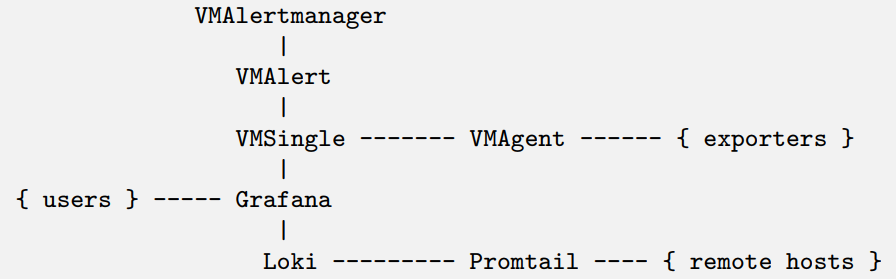
\includegraphics[width=150mm, keepaspectratio]{figures/arch-left.png}
	\caption{System Components}
%	\label{fig:mesh1}
\end{figure}

\subsection{VictoriaMetrics Components}

We are going to use VictoriaMetrics for scraping and storing metrics,
generating alerts and sending out notifications.

As \kszk's infrastructure is small compared to what VictoriaMetrics is able to
handle we have opted for a simple deployment. This type of deployment uses one
service of each type which is easier to configure and handle at the cost of
scalability. We do not expect to hit any bottlenecks with this choice.

\subsubsection{VMAgent}

The VMAgent component pulls metrics from exporters installed on remote hosts.
The list of targets is defined by it's own configuration. Scraped metrics are
then sent to the VMSingle component.

\subsubsection{VMSingle}

The VMSingle component is the central time series database of VictoriaMetrics.
This stores collected metrics and exposes them via an HTTP API. This single
service is basically the cluster version's 3 components (\verb+vminsert+,
\verb+vmstorage+, \verb+vmselect+) compiled into one.

\subsubsection{VMAlert}

The VMAlert component reads metrics from the VMSingle component. Based on it's
configured rules it decides whether the conditions to fire an alert are met. If
an alert fires it is sent to the VMAlertmanager component.

If recording rules are configured it is able to write the results of complex
queries back to VMSingle. This is useful if we want to precalculate time
consuming queries which can later be accessed just like regular metrics.

\subsubsection{VMAlertmanager}

The VMAlertmanager component receives alerts from the VMAlert component. Then
based on it's alert routing and receivers configurations it decides if a
notification should be sent. If conditions are met a notification is sent out
to one or more external services, most importantly to \kszk's Mattermost
(not pictured) server.

\subsection{Promtail}

Promtail receives and processes logs from remote hosts. Unlike VictoriaMetrics
remote hosts push their logs to Promtail. Promtail then sends the processed
logs to Loki.

\subsection{Loki}

Loki indexes and stores logs received from the Promtail component. It receives
requests from Grafana, queries it's internal datastore and responses with the
results. Just like the VictoriaMetrics TSDB Loki can be installed as multiple
instances of different components or as one single component. The former is
useful for higher volumes of logs while the latter is much more simple to set
up and maintain at the cost of scalability. We have opted for the simpler
method as we do not expect to hit any bottlenecks here either.

\subsection{Grafana}

Grafana is only used for visualizations in our architecture. This is our main
user-facing component: users get authenticated and authorized here. After
logging in they are able to create, view and modify dashboards on Grafana.
Grafana queries Loki and/or VMSingle for the data required by the currently
viewed dashboard(s).

%----------------------------------------------------------------------------
\section{Deployment}
%----------------------------------------------------------------------------

All of the above listed components can be installed in a wide variety of ways.
If needed these can be downloaded separately, compiled from source and then run
as classic Unix daemons. Docker images are also available for each of these. On
the other end of the spectrum these components can easily run on Kubernetes as
vast amounts examples, guides and official configurations are available for
this kind of setup.

\subsection{Kubernetes}

Kubernetes\cite{k} is an open-source system for automating the deployment, scaling, and
management of containerized applications. It is a popular platform for running
microservices and other distributed applications, and is often used in
cloud-native environments. Kubernetes provides a number of features to help you
manage your applications, including automatic scheduling and scaling of
containers, self-healing, and service discovery.

We have decied to opt for Kubernetes because:
\begin{itemize}
	\item freely available documentations and configurations make it very easy to use
	\item Kubernetes handles the lifecycle of jobs and pods for us
	\item as \kszk's members already operate a k8s cluster they have experience using this system
	\item by using Kubernetes we can easily expand the system with new physical servers in the future
\end{itemize}

All in all by installing our software stack on Kubernetes we are able to
implement this architecture much quicker, easier and without the need for
custom tools.

%----------------------------------------------------------------------------
% 5. Beszámoló az implementáció folyamatáról
%   - Telepítés során meghozott (rossz) döntések
%   - (rossz) tapasztalatok
%
% A tervezés részletes leírása, a döntési lehetőségek értékelése és a
% választott megoldások indoklása

%\chapter{Introduction}
%\chapter{Earlier monitoring systems implemented in the dormitory}
%\chapter{Requirements of the new monitoring system}
%\chapter{Available industry standard technologies}
%\chapter{System architecture}
\chapter{Implementation details and experiences \label{ch5}}
%\chapter{Results and evaluation}
%\chapter{Future development opportunities}
%----------------------------------------------------------------------------

With the requirements and the system architecture defined we have a clear path
ahead ourselves. There are still quite a few decisions to be made and problems
to be solved. We are going to explore these in this chapter.

%----------------------------------------------------------------------------
\section{The server hardware and the host system}
%----------------------------------------------------------------------------

\subsection{The Hardware}

The hardware was inherited from previous monitoring projects. The machine is a
ProLiant DL360e Gen8 with two Intel Xeon E5-2450L CPUs, 32GBs of RAM, four
Gigabit Ethernet ports, 2x120GB SSDs and 2x1TB HDDs. This should be perfect to
serve our needs.

\subsection{The Operating System}

For the host operating system we are going to use a Linux distribution aimed at
servers. We have several choices here favouring ones that \kszk already
operate. These are: Ubuntu, Debian and Rocky Linux.

Ubuntu is developed and maintained by Canonical, a UK-based company. It had
been a popular choice among desktop and server Linux users alike. Unfortunately
it's most recent developments such as snaps made many previous users dislike
this system and migrate to others.

Debian is developed and maintained by a community of volunteers from around the
world. It is known for its stability and reliability, making it a popular
choice for servers and other mission-critical systems. It also has a large
repository of pre-compiled software packages, making it easy to install and
manage applications. Ubuntu is also based on Debian.

Rocky Linux is based on the codebase of Red Hat Enterprise Linux (RHEL), but is
developed and maintained by a community of volunteers. It aims to provide a
secure and stable platform that is compatible with RHEL, while also being free
of any vendor restrictions or licensing fees. It also comes with SELinux
preconfigured, making it more secure.

\subsection{The Kubernetes Distribution}

As for a Kubernetes distribution we of course have k8s. K8s supports everything
we need, however it is aimed at larger installations and multi-node clusters
thus it is harder to configure and more resource-intensive. A better
alternative is k3s, which is a lightweight, open-source Kubernetes distribution
that is designed to be easy to install and operate on resource-constrained
environments, such as edge computing or IoT devices. K3s also supports SELinux
and works perfectly with Rocky Linux.

\subsection{The Final Host System Configuration}

For the above reasons we decided to use Rocky Linux as the host OS, k3s as the
Kubernetes distribution and we are going to install VictoriaMetrics and Grafana
on top of these.

We installed the host system on the two SSDs configured as Linux Software RAID1
for redundancy and better uptime. The data is going to be stored on the two
HDDs for which we used ZFS and the HDDs are configured as a two-way mirror
(equivalent to a RAID1 in redundancy).

ZFS supports many advanced features besides different redundancy levels such as
encryption, checksumming, compression and snapshots. Although we do not yet
make use of these we have the opportunity to enable them in the future without
worrying about migration of the system which would couse unnecessary downtime.

Another issue we need to take care of is reproducibility. As setting up such a
system takes much time, effort and research it's not enough to only document
this progress. During migration to new hardware (in case of an upgrade or a
catastrophical failure) we would have to repeat all this work. To solve this we
chose to use Ansible which is already widely used by \kszk.

Ansible is an open-source IT automation tool that allows users to configure and
manage systems, deploy applications, and automate processes. It uses YAML files
just like the rest of our tools, and then uses a series of modules to enforce
that state on the system.

Every change is going to be applied through Ansible and every file used is
going to be stored on a repository on \kszk's GitLab server.

%----------------------------------------------------------------------------
\section{Preparing the k3s Kubernetes distribution}
%----------------------------------------------------------------------------

On it's own, Kubernetes is a very powerful tool. It can handle many containers,
services, load balancers and much more. But even a single pod contains at least
one docker container. It's configuration is managed via YAML files but this way
of management becomes repetitive very quickly (imagine repeating the same port
numbers over many configuration files) violating the DRY (Don't Repeat
Yourself) principle and becomes a nightmare to maintain. To overcome this issue
the community had created several tools to ease it's use.

\subsection{Management Tools}

The k3s kubernetes distribution can be managed the same way as it's
heavywheight, full-fledged k8s brother. Thus we are going to use the same tools
we'd use on a more complicated deployment.

Managing a kubernetes cluster can be (and I usually done) remotely. By this I
don't mean an SSH session - the Kubernetes command-line tool, \verb+kubectl+
tool runs on any administrator's machine and for authentication we need to copy
the \verb+/etc/rancher/k3s/k3s.yaml+ configuration file from the k3s host
machine.

Now we have the power to manage our cluster yet this does not free us from
writing complicated, thousands-of-lines long YAML configuration files for
deployment. The solution is Helm.

Helm is an open-source package manager for Kubernetes that allows users to
easily install, upgrade, and manage applications on Kubernetes clusters. Helm
uses a packaging format called charts, which are pre-configured templates that
define the desired state of an application, including its dependencies,
configuration, and resources.

\subsection{Persistent Volumes}

VictoriaMetrics' and Loki's stateful components are going to need a persistent
volume which we want to store on our ZFS mirror. Persistent volumes are going
to be provided by the OpenEBS ZFS CSI Driver. Installation is easy:
\verb+kubectl apply -f https://openebs.github.io/charts/zfs-operator.yaml+.

We have to configure the driver to use our pool.

\begin{lstlisting}[language=yaml,caption=zfs-localpv.sc.yaml]
apiVersion: storage.k8s.io/v1
kind: StorageClass
metadata:
  name: openebs-zfspv
parameters:
  recordsize: "4k"
  compression: "off"
  dedup: "off"
  fstype: "zfs"
  poolname: "spinningrust/openebs-zfspv"
provisioner: zfs.csi.openebs.io
\end{lstlisting}

Configuration is applied yet again by the following command:
\verb+kubectl apply -f zfs-localpv.sc.yaml+.

% install krew for kubectl
% install minio for kubectl

%----------------------------------------------------------------------------
\section{Installing and configuring a basic VictoriaMetrics on k3s}
%----------------------------------------------------------------------------

Now that we have set up k3s we can begin installing and configuring
VictoriaMetrics.

Before we continue let's take a look at how Helm works. Complex, multi-pod
kubernetes systems are set up by many large YAML files. These files contain
redundant informations, hard to comprehend and difficult to work with. Helm
uses template files (which use Go syntax) which handle everything that can be
computed, and so called values files. The latter contain sane default
configurations where such things make sense and require the user to enter
values where no such configurations can exist, for example external services'
authentication details. The combination of these is called a helm chart. Helm
charts can be added to the system manually or by adding a helm chart
repository.

\subsection{Downloading the Helm Charts}

First of all we are going to add the VM helm chart repository following the
intructions on VM's GitHub repository:
\url{https://github.com/VictoriaMetrics/helm-charts}.

\begin{lstlisting}
helm repo add vm https://victoriametrics.github.io/helm-charts/
helm repo update
\end{lstlisting}

Next, we are going to select the helm chart that fits our needs. The repository
contains many charts most of which only contain a subset of a full
VictoriaMetrics stack. The one we need is \verb+victoria-metrics-k8s-stack+,
this is the full k8s VM stack.

Before installing this we have to configure it through the correct values file.
We can get the values file with the help of the \verb+helm show values+
command:

\begin{lstlisting}
helm show values vm/victoria-metrics-k8s-stack > values.yaml
\end{lstlisting}

For the initial \verb+values.yml+ see Appendix~\ref{vmValues}.

\subsection{Installing VictoriaMetrics}

Once the \verb+values.yml+ is configured the helm chart is installed with the
following command:

\begin{lstlisting}
helm install beholder vm/victoria-metrics-k8s-stack -f values.yml
\end{lstlisting}

%----------------------------------------------------------------------------
\section{Collecting metrics}
%----------------------------------------------------------------------------

With VictoriaMetrics up and running we can begin collecting our metrics from
various servers and network devices. In fact, we are already collecting some
metrics: the helm chart used before already configured the monitoring of
VictoriaMetrics, k3s and the host node itself.

The stack installed also contains another powerful feature: the VictoriaMetrics
Kubernetes Operator.

An operator is a piece of software that extends the Kubernetes API to create,
configure, and manage instances of complex applications. This allows you to use
the Kubernetes API to automate tasks such as deploying, scaling, and backing up
your applications. They provide a declarative way to describe the desired state
of an application, and then automatically reconciling the actual state of the
application with the desired state.

\subsection{Collecting Metrics from Servers}

We are going to add 3 servers for demontration purposes:
\begin{itemize}
	\item memory-alpha and memory-beta: this is a ZFS-based storage server cluster
	\item trash: this server provides music for \kszk's hard-working members
\end{itemize}

To collect metrics from a remote system the target host must have the
neccessary exporters installed and configured. Exporters are a piece of
software that collect metrics from system components and expose them throug an
HTTP API. Different kinds of exporters collect different metrics: the generic
node exporter collect basic statistics such as CPU and RAM usage, while
specialized exporters are needed to collect metrics from components such as
ZFS, mailing servers or databases.

After the desired exporters are installed and configured on the target host we
have to inform VictoriaMetrics about their existence. For this we have to
define \verb+VMStaticScrape+ objects, apply these configurations and let the
operator configure the \verb+vmagnet+ component to collect metrics from these
servers as well. The configuration is as follows:

\begin{lstlisting}[language=yaml,caption=Configuration file for memory-alpha and memory-beta]
apiVersion: operator.victoriametrics.com/v1beta1
kind: VMStaticScrape
metadata:
  name: memory-alpha-and-beta
  namespace: monitoring
spec:
  targetEndpoints:
    - targets:
        - 10.0.69.101:9100
        - 10.0.69.102:9100
  jobName: memory-alpha-and-beta
\end{lstlisting}

\begin{lstlisting}[language=yaml,caption=Configuration file for trash]
apiVersion: operator.victoriametrics.com/v1beta1
kind: VMStaticScrape
metadata:
  name: trash
  namespace: monitoring
spec:
  targetEndpoints:
    - targets:
        - 152.66.209.79:9100
  jobName: trash
\end{lstlisting}

The \verb+.metadata.name+ and \verb+.metadata.namespace+ values identify the
resouce, while key-value pairs under the \verb+.spec+ key define the
configuration itself. The \verb+.spec.targetEndpoints.targets+ array contain
the ip+port pairs for every available exporter, while \verb+.spec.jobName+ is
used to locate the collected metrics inside \verb+vmagent+ and \verb+Grafana+.

These files contain many boilerplate around little information. Luckily we have
a solution for this which we going to explore in the next section.

The monitoring server has a dedicated interface in the administration VLAN just
like every other server operated by \kszk - this means that we can reach these
targets directly.

\subsection{Collecting Metrics from Network Devices}

Monitoring network devices is slightly more complicated.  Network devices can
not run arbitrary softwares such as exporters and these devices can only be
reached on a physically separated network knowns as the management LAN. Luckily
we can reach the NOCs (Network Operation Centers) which are connected to this
network. For the other part we must use some kind of exporter that runs
separately and collects data through SNMP.

The Prometheus project has a solution exactly for this:
\url{https://github.com/prometheus/snmp_exporter/tree/main/generator} and \kszk
already has an SNMP exporter with the required MIBs built in. We installed one
instance of this exporter on each NOC. The exporters are reached through a k3s
loadbalancer, this makes sure that the metrics are not duplicated and so far at
least one exporter is running metrics are going to be collected.

\begin{lstlisting}[language=yaml,caption=Load balancer configuration]
apiVersion: v1
kind: Service
metadata:
  name: noc-snmp-exporter
spec:
  ports:
    - port: 80
      targetPort: 9116
      name: exporter
      protocol: TCP
  type: ClusterIP

---
apiVersion: v1
kind: Endpoints
metadata:
  name: noc-snmp-exporter
subsets:
  - ports:
      - port: 9116
        name: exporter
        protocol: TCP
    addresses:
      - ip: 10.0.208.241
      - ip: 10.0.208.242
\end{lstlisting}

With all these set up we can scrape network devices just like we did with
servers. Below is showed the initial configuration scraping the core router
\verb+rtr-1+ only.

\begin{lstlisting}[language=yaml,caption=Initial SNMP scraping configuration]
apiVersion: operator.victoriametrics.com/v1beta1
kind: VMStaticScrape
metadata:
  name: schnet-snmp
  namespace: monitoring
spec:
  jobName: schnet-snmp
  targetEndpoints:
    - targets:
        - noc-snmp-exporter:80
      path: /snmp
      params:
        target: [ rtr-1 ]
        module: [ sch_core_net_mibs ]
\end{lstlisting}

Note that all network device metrics are reached through a single exporter. The
\verb+.spec.targetEndpoints.params.target+ key identifies the device.

\subsection{Metric Visualizations}

As for visualization, our \verb+Grafana+ comes with some common dashboards
preinstalled such as a node exporter, kubernetes exporter and VictoriaMetrics
dashboards. Other, commonly used dashboards can easily be imported from
\url{https://grafana.com/grafana/dashboards/}. Unique dashboards, such as the
ones displaying our SNMP metrics must be created by us.

\begin{figure}[!h]
	\centering
	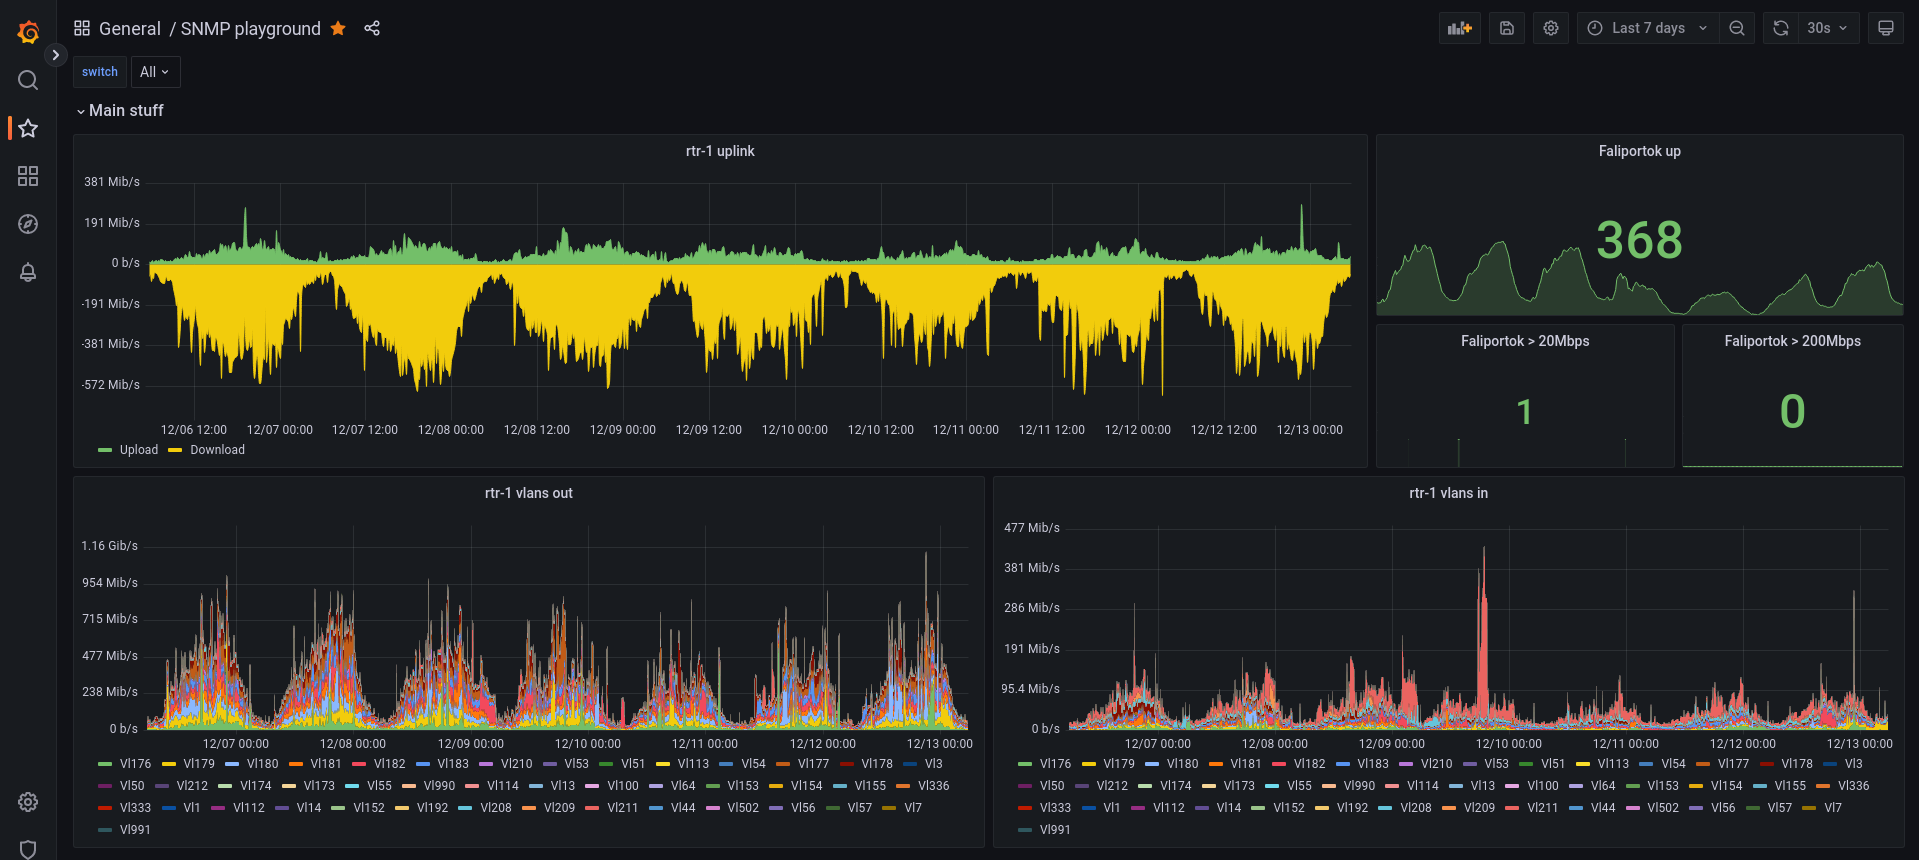
\includegraphics[width=150mm, keepaspectratio]{figures/grafana-snmp-playground.png}
	\caption{Screenshot of the Grafana SNMP Playground Dashboard at the time of writing}
\end{figure}

The above is shown a screenshot of the SNMP Playground dashboard. After the
initial version was released members of \kszk took their time and added many
other useful metrics to this visualization. The 'Faliportok up' panel shows
every active 1Gbit endpoint on the \sch's network. It shows nicely the least
actively used periods of the week: between 4am and 8am especially on the
weekends.

%----------------------------------------------------------------------------
\section{Automating tasks with the help of GitLab CI}
%----------------------------------------------------------------------------

Now we are able to monitor our servers and network devices. However as seen
above, configuration is very repetitive. Moreover, adding or modifiny any
device requires the contribution of the monitoring system administrator which
slows down the integration and wastes time that could be utilized better
elsewhere.

We already have a perfect tool for generating configurations: helm charts. We
can quickly and easily create simple ones ourselves. For defining a helm chart
we need:

\begin{itemize}
	\item \verb+./Chart.yaml+: this contains some required metadata about the chart itself
	\item \verb+./template/*.yaml+: these are the Go templates themselves, the final config will be generated from these files
	\item \verb+./template/*.tmpl+: these are helper template functions
	\item \verb+./values.yaml+: the values for the template
\end{itemize}

\subsection{Implementing Helm Charts for Configuration Generation}

Let's review the implementation of the node exporter helm chart.

\begin{lstlisting}[language=yaml,caption=./Chart.yaml]
apiVersion: v2
name: node-exporter-target
description: Scrape configs for Prometheus node exporter
type: application
version: 0.0.0
appVersion: "kolbaasz"
\end{lstlisting}

\begin{lstlisting}[language=yaml,caption=./templates/\_helpers.tmpl]
{{- define "name" }}
{{- .Chart.Name }}-{{.Release.Name}}
{{- end }}
\end{lstlisting}

\begin{lstlisting}[language=yaml,caption=./templates/node-exporter.yaml]
{{- $global := . }}
{{- range .Values.Devices }}
---
apiVersion: operator.victoriametrics.com/v1beta1
kind: VMStaticScrape
metadata:
  name: "{{ template "name" $global }}-{{ .Name }}"
  namespace: monitoring
spec:
  targetEndpoints:
    - targets:
        {{- range .Targets }}
        - "{{ . }}"
        {{- end }}
  jobName: "{{ .Name }}"
{{- end }}
\end{lstlisting}

\begin{lstlisting}[language=yaml,caption=./values.yaml]
Devices:
  - Name: memory-alpha-and-beta
    Targets:
      - 10.0.69.101:9100
      - 10.0.69.102:9100

  - Name: trash
    Targets: [ 152.66.209.79:9100 ]
\end{lstlisting}


These Go templates operate with the values file in context as \verb+.Values+.
This chart iterates over the \verb+.Values.Devices+ array's elements with the
\verb+range+ function, creates a \verb+VMStaticScrape+ object for each one.
Each \verb+VMWStaticScrape+'s \verb+.spec.targetEndpoints.targets+ array is
filled with the matching \verb+.Values.Devices.Targets+ array's elements.

Now when adding a new device the administrator only has to edit the
\verb+values.yml+ file which now only contains the neccessary informations
without any noise.

To start using this new method, first we have to install the helm chart:
\verb+helm install -n monitoring node-exporter-targets .+. For subsequent uses
we can upgrade the chart: \verb+helm upgrade -n monitoring node-exporter-targets .+.

We can generate SNMP monitoring configurations the same way. See the helm chart
in Appendix~\ref{snmpScraperChart}.

\subsection{Configuring GitLab CI}

We had achieved a way to write monitoring configurations easily but this
approach still requires the intervention of a precious sysadmin. Countionous
integration is our way to go. Our repository on \kszk's GitLab contains
everything needed to add new hosts to the system, let's make use of GitLab's
Contionous Integration (CI) features. For this the following
\verb+.gitlab-ci.yml+ file is going to be used.

\begin{lstlisting}[language=yaml,caption=.gitlab-ci.yml]
stages: [ sanity_check, upgrade_charts ]

before_script:
  - apk add diffutils
  - kubectl config use-context kszk/ansible/playbooks/monitoring:beholder

node_check:
  stage: sanity_check
  image: alpine/k8s:1.24.8
  script:
    - ./helmdiff.sh node-exporter-targets ./files/helm-charts/node-exporter-target
  only:
    changes:
      - files/helm-charts/node-exporter-target/**
      - .gitlab-ci.yml
      - helmdiff.sh

snmp_check:
  stage: sanity_check
  image: alpine/k8s:1.24.8
  script:
    - ./helmdiff.sh snmp ./files/helm-charts/snmp-exporter-target
  only:
    changes:
      - files/helm-charts/snmp-exporter-target/**
      - .gitlab-ci.yml
      - helmdiff.sh

node_export:
  stage: upgrade_charts
  image: alpine/k8s:1.24.8
  script:
    - helm upgrade -n monitoring node-exporter-targets ./files/helm-charts/node-exporter-target
  only:
    changes:
      - files/helm-charts/node-exporter-target/**
      - .gitlab-ci.yml
      - helmdiff.sh
    refs:
      - main

snmp_export:
  stage: upgrade_charts
  image: alpine/k8s:1.24.8
  script:
    - helm upgrade -n monitoring snmp ./files/helm-charts/snmp-exporter-target
  only:
    changes:
      - files/helm-charts/snmp-exporter-target/**
      - .gitlab-ci.yml
      - helmdiff.sh
    refs:
      - main
\end{lstlisting}

Note the \verb+helmdiff.sh+ script used above. We tried to use the already
available helm diff plugin but ran into several problems, the version we used
did not accept our new and completely valid configurations. For this reason we
used the following script:

\begin{lstlisting}[language=bash,caption=helmdiff.sh]
#!/bin/sh

set -ueo pipefail

release="$1"
chart="$2"

helm get manifest -n monitoring "$release" > /tmp/installed
helm template -n monitoring "$release" "$chart" > /tmp/new

diff -w --color=always -y /tmp/installed /tmp/new || [ "$?" = "1" ]
\end{lstlisting}

The CI scripts run on the monitoring server in docker inside an Alpine image.
The image is complemented with the \verb+diffutils+ package which is required
by the \verb+helmdiff.sh+ script. The CI runs on two stages for each of our
helm charts. The first stage, \verb+sanity_check+ verifies the syntactic
validity of our new configuration as well as displays the difference between
the current and the newly generated difference using \verb+helmdiff.sh+. On the
main branch the \verb+upgrade_charts+ stage upgrades our helm charts using the
new configurations. One job per helm chart is used in each stage and each job
is only ran when neccessary (i.e. when a change was made).

Using these tools new systems can be monitored with minimal knowledge and
without the intervention of a monitoring system administrator.

%----------------------------------------------------------------------------
\section{Authentication and authorization}
%----------------------------------------------------------------------------

So far our users can set up monitoring for any of their devices but we are far
from done. As only the hardcoded \verb+Administrator+ account can log into the
otherwise publicly available Grafana users can not make use of the system.

We are going to authenticate and authorize our users through AuthSCH with OAuth
2.0. Luckily Grafana supports this protocol. Unlucky for us Grafana expects the
user's e-mail to be at the \verb+/email+ path exactly and we found no way to
reconfigure this. For legacy reasons AuthSCH serves the e-mail in a different
path.

To work around this issue we created a very simple proxy server that translates
AuthSCH's response to the format expected by Grafana. Since the implementation
of this service is trivial we are not going to explore this further.

\begin{lstlisting}[language=yaml,caption=Grafana OAuth 2.0 configuration]
grafana:
  grafana.ini:
    auth.generic_oauth: # client is at Garmine's SCHAcc
      name: "AuthSCH"
      enabled: "true"
      client_id: "18023005984133885935"
	  client_secret: "secret" # Redacted for security purposes
      scopes: "basic displayName admembership linkedAccounts"
      auth_url: "https://auth.sch.bme.hu/site/login"
      token_url: "https://auth.sch.bme.hu/oauth2/token"
      api_url: "http://authsch-api-authsch.authsch-hack.svc/grafana" # ha-ha
      allow_sign_up: "true"
      role_attribute_path: "contains(adgroups[*], 'KSZK') && 'Admin' || contains(adgroups[*], 'KSZKUjonc') && 'Viewer' || 'Vesztettem'"
      role_attribute_strict: "true"
      groups_attribute_path: "adgroups"
\end{lstlisting}

The above is a pretty standard OAuth 2.0 configuration. Notable are the
different \verb+api_url+ path (these requests are routed through our proxy) and
the \verb+role_attribute_path+ value. The latter describes the authorization
based on AD group memberships. Members of the \verb+KSZK+ group are granted
\verb+Admin+ role: they are authorized to do make any changes in Grafana save
for a few things such as managing users and changing permissions. Members of
the \verb+KSZKUjonc+ group are granted \verb+Viewer+ role: they are authorized
to view almost any part of our Grafana but can not make any changes. Other
users would get \verb+Vesztettem+ which is a nonexsistent role, thus they are
denied logging in.

Superadmin rights are granted locally either through the above mentioned
\verb+Administrator+ account or by another superadmin account.

%----------------------------------------------------------------------------
\section{Collecting logs}
%----------------------------------------------------------------------------

\subsection{Configuring and Installing Loki}

We are going to use Loki for writing, storing and querying logs. Loki just like
VictoriaMetrics can be split into smaller services and installed in a larger,
distributed and scalable form as a cluster for heavier workloads. For smaller
infrastructures Loki can be installed as a single service as well which is
easier to configure and should fit our needs perfectly. For this we are going
to write Loki's \verb+loki-values.yml+ file.

First of all we are going to install the helm chart as before:

\begin{lstlisting}[language=bash,caption=Installing Loki's helm chart]
helm repo add grafana https://grafana.github.io/helm-charts
helm repo update
\end{lstlisting}

\begin{lstlisting}[language=yaml,caption=loki-values.yml]
loki:
  commonConfig:
    replication_factor: 1
  storage:
    type: filesystem
  server:
    log_level: warn

monitoring:
  selfMonitoring:
    enabled: false

test:
  enabled: false

write:
  replicas: 0

read:
  replicas: 0

singleBinary:
  replicas: 1
  persistence:
    size: 256Gi
    storageClass: openebs-zfspv

ingress:
  enabled: false

gateway:
  enabled: false

networkPolicy:
  enabled: false

minio:
  enabled: false
\end{lstlisting}

In order to configure Loki as a single binary we need a single replica of
\verb+singleBinary+ and no \verb+write+ and \verb+read+ replicas. Logs are
going to be stored on a persistent volume provided by \verb+openebs-zfspv+. For
now we are going to disable selfmonitoring and testing as well.

Once the configuration is ready we are going to install as usual:
\verb+helm install --values loki-values.yaml loki grafana/loki+

Loki only receives logs from another service and does no processing on them. In
order to send logs to Loki we are going to use Promtail. Promtail is very
versatile, is able to receive and collect logs from various sources and can
process the logs before sending them. We are going to split the responsibility
of collecting and processing logs. Logs are going to be collected and sent by
the hosts themselves either via Promtail (for servers) or syslog (for more
simple devices such as routers and switches). Processing the logs is going to
be done by a Promtail instance running on the monitoring system. This way
target hosts can send logs with minimal and very simple configurations while
the monitoring system administrators can configure log processing locally,
without having access to the target hosts.

\subsection{Collecting Logs of the Monitoring System}

The first target for log collecting is the monitoring system itself. So far
only the system administrators had access to these logs via the
\verb+kubectl logs+ command. Having access to these logs would make debugging
much easier for our users.

\begin{lstlisting}[language=yaml,caption=local-promtail-values.yml]
daemonset:
  enabled: false

deployment:
  enabled: true
  replicaCount: 1

serviceMonitor:
  enabled: true

config:
  logLevel: warn
  serverPort: 3101
  clients:
    - url: http://loki:3100/loki/api/v1/push
  snippets:
    common:
      - action: replace
        target_label: job
        replacement: beholder-pods
\end{lstlisting}

The local Promtail's configuration is changed minimally: since we are running a
single node kubernetes cluster we opt for a single replica deployment,
\verb+serviceMonitor+ is enabled for the VictoriaMetrics operator and collected
logs' are stored under the `beholder-pods` job for easy identification.

\subsection{Receiving and Processing Logs from other Systems}

The other Promtail instance is going to receive, process and then send the
remotely collected logs to Loki. Let's take a look at it's configuration.

\begin{lstlisting}[language=yaml,caption=promtail-values.yml]
daemonset:
  enabled: false

deployment:
  enabled: true
  replicaCount: 1

defaultVolumes: []
defaultVolumeMounts: []

serviceMonitor:
  enabled: true

extraPorts:
  syslog:
    name: tcp-syslog
    containerPort: 1514
    protocol: TCP
    externalTrafficPolicy: Local
    service:
      type: ClusterIP # TODO make LoadBalancer after auth has been figured out
      port: 1514
  promhttp:
    name: prom-http
    containerPort: 3500
    protocol: TCP
    service:
      type: ClusterIP
      port: 3500
  promgrpc:
    name: prom-grpc
    containerPort: 3600
    protocol: TCP
    service:
      type: ClusterIP
      port: 3600

config:
  file: |
    server:
      log_level: info
      http_listen_port: 3101
    clients:
      - url: http://loki:3100/loki/api/v1/push

    positions:
      filename: /run/promtail/positions.yaml

    scrape_configs:
      - job_name: syslog
        syslog:
          listen_address: 0.0.0.0:1514
          labels:
            job: syslog
        relabel_configs:
          - source_labels: [ __syslog_message_hostname ]
            target_label: host
          - source_labels: [ __syslog_message_severity ]
            target_label: severity
          - source_labels: [ __syslog_message_facility ]
            target_label: facility
          - source_labels: [ __syslog_message_app_name ]
            target_label: app
            
      - job_name: prom
        loki_push_api:
          server:
            http_listen_port: 3500
            grpc_listen_port: 3600
          labels:
            job: prom

    limits_config: {}
\end{lstlisting}

Similarly to the local Promtail we opt for a single replica deployment. As we
do not with to collect local logs with this instance we disable
\verb+defaultVolumes+ and \verb+defaultVolumeMounts+. The \verb+extraPorts+ map
configures Promtail to accept connections from syslog and other Promtail
instances. The \verb+config.file+ is just a string, literally the contents of
Promtail's configuration file. The above is just a simple forwarding for
Promtail and syslog, with added label translation for syslog.

Installation is done with \verb+helm install+ for both charts just as before.

For demonstration purposes we installed a Promtail instance on a server called
\verb+trash+. After setting up a Grafana dashboard we are able to successfully
browse \verb+trash+'s logs.

\newpage

\subsection{Log Visualization}

\begin{figure}[!h]
	\centering
	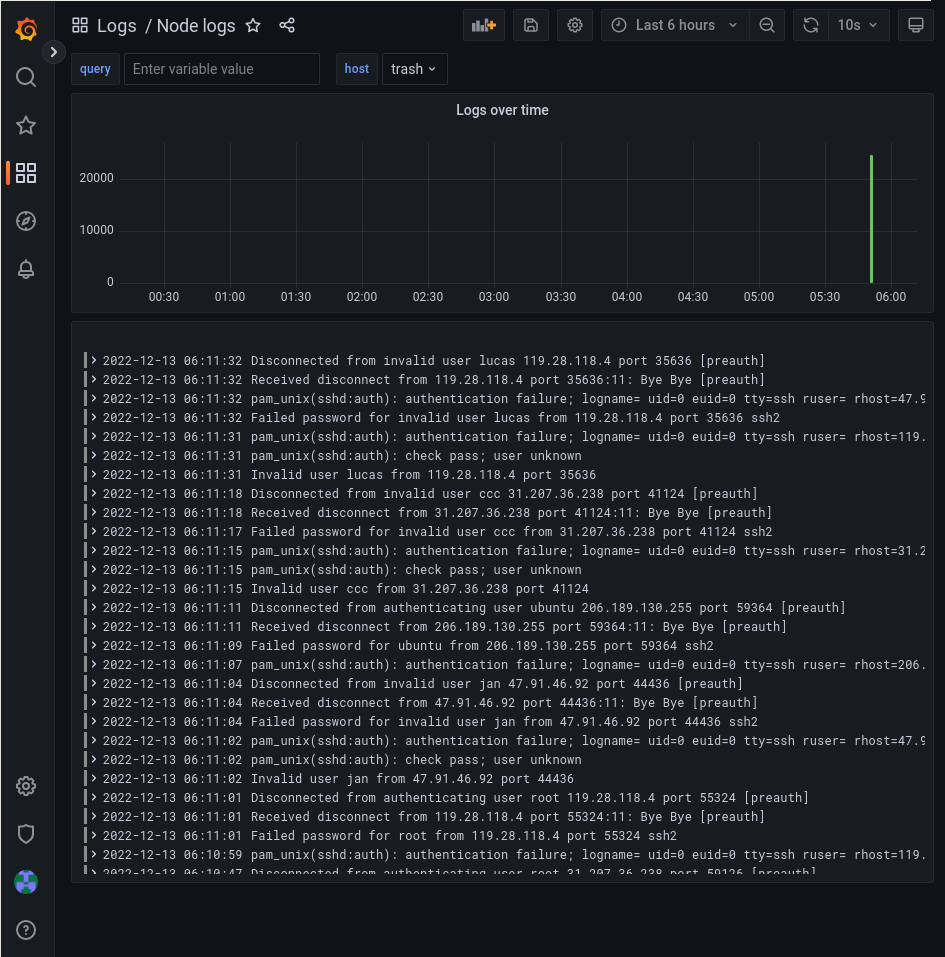
\includegraphics[width=150mm, keepaspectratio]{figures/grafana-logs-trash.png}
	\caption{Screenshot of the Grafana Logs dashboard just after implementation}
\end{figure}

Above is seen a screenshot of the Grafana Logs dashboard. On the logs collected
from Trash, \kszk's media-player VM we can see several unsuccessful log-in
attempts from various botnets.

\subsection{Security}

For security purposes authentication is mandatory for receiving logs. Both
Promtail->Promtail and syslog->Promtail ways are able to use authentication. As
many network devices don't support anything else than sending logs via
unauthenticated and unencrypted syslog we have postponed this feature.

%----------------------------------------------------------------------------
\section{Creating alerts and sending notifications}
%----------------------------------------------------------------------------

In the monitoring stack the \verb+vmalert+ component communicates with the
VictoriaMetrics TSDB, has access to every metric and executes recording and
alerting rules. Recording rules' results are written back to the TSDB while
alerting rules send notifications to the \verb+vmalertmanager+ component. The
alert manager then routes these alerts to various receivers. Receivers then
finally format and send out alerts to external platforms. These include but are
not limited to: e-mail, Slack API, Telegram and HTTP.

\subsection{Configuring VMAlert}

Our \verb+vmalert+ configuration is very plain. The bulk of it's configuration,
the alerting and recording rules are applied through the VictoriaMetrics
kubernetes operator.

\begin{lstlisting}[language=yaml,caption=vmalert configuration]
vmalert:
  annotations: {}
  enabled: true
  spec:
    selectAllByDefault: true
    image:
      tag: v1.83.0
    evaluationInterval: 15s

  templateFiles:
    {}

  ingress:
    enabled: false
\end{lstlisting}

Luckily the kubernetes VictoriaMetrics stack comes with a plethora of alerting
rules preconfigured. Some of these alerts only fire on VictoriaMetrics' error
conditions while others are applied for every monitored node such as NTP out of
sync and RAID error alerts.

\begin{lstlisting}[language=yaml,caption=Example alerting rule configuration]
apiVersion: operator.victoriametrics.com/v1beta1
kind: VMRule
metadata:
  name: beholder-victoria-metrics-k8s-stack-node-exporter
  namespace: monitoring
spec:
  groups:
  - name: node-exporter
    rules:
    - alert: NodeClockSkewDetected
      annotations:
        description: Clock is out of sync by more than 300s. Ensure NTP is configured correctly on this host.
        runbook_url: https://runbooks.prometheus-operator.dev/runbooks/node/nodeclockskewdetected
        summary: Clock skew detected.
      expr: |-
        ( node_timex_offset_seconds >  0.05 and deriv(node_timex_offset_seconds[5m]) >= 0 )
        or
        ( node_timex_offset_seconds < -0.05 and deriv(node_timex_offset_seconds[5m]) <= 0 )
      for: 10m
      labels:
        severity: warning
\end{lstlisting}

The above is an example for alerting when the system clock drifts more than 300
seconds on any monitored node.

\subsection{Configuring VMAlertmanager}

These alerting rules are ideal for demonstration purposes and are also useful
for real-life scenarios. But with nowhere to go they would be worthless, so
let's configure our alert manager to send everything to \kszk's Mattermost
server's \verb+~alerts-test+ channel for now.

\begin{lstlisting}[language=yaml,caption=alertmanager configuration]
alertmanager:
  enabled: true
  spec:
    selectAllByDefault: true
    externalURL: ""
    routePrefix: /

  config:
    global:
      resolve_timeout: 5m
	  slack_api_url: "https://127.0.0.1" # Redacted for security reasons

    templates:
      - "/etc/vm/configs/**/*.tmpl"
    route:
      group_by: ["alertgroup", "job"]
      group_wait: 30s
      group_interval: 5m
      repeat_interval: 12h
      receiver: "mattermost"

    receivers:
      - name: "mattermost"
        slack_configs:
          - channel: "#alerts-test"
            username: "SCP-049"
            send_resolved: true
            title: '{{ template "slack.monzo.title" . }}'
            icon_emoji: '{{ template "slack.monzo.icon_emoji" . }}'
            color: '{{ template "slack.monzo.color" . }}'
            text: '{{ template "slack.monzo.text" . }}'
            actions:
              - type: button
                text: "Runbook :green_book:"
                url: "{{ (index .Alerts 0).Annotations.runbook_url }}"
              - type: button
                text: "Dashboard :grafana:"
                url: "{{ (index .Alerts 0).Annotations.dashboard }}"
              - type: button
                text: "Silence :no_bell:"
                url: '{{ template "__alert_silence_link" . }}'

  # better alert templates for slack
  # source https://gist.github.com/milesbxf/e2744fc90e9c41b47aa47925f8ff6512
  monzoTemplate:
    enabled: true

  templateFiles:
    {}

  ingress:
    enabled: false
\end{lstlisting}

Mattermost uses the Slack API for incoming webhooks. This sample
\verb+alertmanager+ config uses trivial routing. A single failure usually
triggers more alerts at once so it only tries to send alerts as a batch in a
single message instead of one-by-one in order to reduce noise. The receiver
config on the other hand hilights some nice features:

\begin{itemize}
	\item we receive a notification when the cause is fixed
	\item the monzo templates nicely decorate the message
	\item we get a button to the relevant runbook (basically a manual for the alert)
	\item we get a button to the relevant Grafana Dashboard
	\item we get a button that silences the alert
\end{itemize}

\newpage

\subsection{Alerts on Mattermost}

After applying the new configuration using \verb+helm upgrade+ we instantly
receive several alerts on Mattermost's \verb+~alerts-test+ channel that had
been stuck in the queue.

\begin{figure}[!h]
	\centering
	
\includegraphics[width=150mm, keepaspectratio]{figures/mattermost-alert-x-ray.png}
	\caption{Screenshot of a real alert on \kszk's Mattermost server}
\end{figure}

Above is shown a real alert sent from VictoriaMetrics to \kszk's Mattermost
server. This alert unexpectedly unveiled a real problem: one of our servers
system clock did not properly synchronise via NTP. The difference was around
500 milliseconds.

As it turns out the Mattermost API is not 100\% compatible with Slack's: even
though both support interactive messages and buttons we do not get them with
the alert messages.

\subsection{Implementing Continous Integration for Alerts}

Even though the preconfigured alerts are useful we want to give out users the
ability to define their own alerts. For this we are going to use GitLab CI as
well.

Ideally we would have a single helm chart for everything: monitoring, logging
and alerting configurations. This would eliminate every repetition and with a
preconfigured rules library would make alerting much more simple. This would
require lots of work and careful planning. This is out of the scope for this
project and thus we have opted for a much more trivial solution. See the helm
chart for adding alerting and recording rules in
Appendix~\ref{snmpScraperChart}.

We installed the helm chart usnig the \verb+helm install+ command and added the
following new jobs to \verb+.gitlab-ci.yml+

\begin{lstlisting}[language=yaml,caption=New jobs in .gitlab-ci.yml]
alerts_check:
  stage: sanity_check
  image: alpine/k8s:1.24.8
  script:
    - ./helmdiff.sh kszk-alerts ./files/helm-charts/kszk-alerts
  only:
    changes:
      - files/helm-charts/kszk-alerts/**
      - .gitlab-ci.yml
      - helmdiff.sh

alerts_upgrade:
  stage: upgrade_charts
  image: alpine/k8s:1.24.8
  script:
    - helm upgrade -n monitoring kszk-alerts ./files/helm-charts/kszk-alerts
  only:
    changes:
      - files/helm-charts/kszk-alerts/**
      - .gitlab-ci.yml
      - helmdiff.sh
    refs:
      - main
\end{lstlisting}

Although it's more complicated than ideal we gave our users the tools
neccessary to configure their own alerting and recording rules without the
intervention of a monitoring system administrator.

%----------------------------------------------------------------------------
% 6. A futó rendszer értékelése
%   - Összevetés a követelményekkel
%   - Pro/contra, jó és rossz tapasztalatok
%
% A megtervezett műszaki alkotás értékelése, kritikai elemzése

%\chapter{Introduction}
%\chapter{Earlier monitoring systems implemented in the dormitory}
%\chapter{Requirements of the new monitoring system}
%\chapter{Available industry standard technologies}
%\chapter{System architecture}
%\chapter{Implementation details and experiences}
\chapter{Results and evaluation \label{ch6}}
%\chapter{Future development opportunities}
%----------------------------------------------------------------------------

During the time of writing the monitoring system has been running for months
now with gradually increasing capabilities as time went on. Although most
requirements were met the system is still in development. Let's take a look at
the current state of it.

%----------------------------------------------------------------------------
\section{Evaluation of Requirements Fulfillment}
%----------------------------------------------------------------------------

The most important is meeting the requirements laid out in \autoref{ch2}.

\subsection{Collecting and storing metrics and logs}

The currently installed system is more than capable of collecting and storing
metrics and logs. We are able to monitor every server platform and network
device currently in use by \kszk.

At the time of writing many systems including Windows Servers, Linux Servers
and Cisco devices are already being monitored. Only logs are not being
collected from network devices due to debates about an optimal and secure
solution.

\subsection{Effective long-term storage of historical data}

The system is currently capable of storing data for short to mid terms. The
implementation of long-term storage was least concern. With proper
configuration such as fine tuned retentions and external storage both
VictoriaMetrics and Loki are able to effectively storage large amounts of data
only limited by available storage.

\subsection{Detecting issues and alerting the necessary personnel}

VictoriaMetrics' components already detect some basic issues and send out
alerts to a test channel on \kszk's Mattermost platform. The software stack is
capable of detecting much more complex issues and sending out alerts on many
communications channels. This perfectly demonstrates our top priority:
preventing future issues and detecting existing ones.

\subsection{Detecting issues of the monitoring system itself (meta-monitoring)}

Meta-monitoring is partially implemented. The system collects and visualizes
many metrics and logs about itself as well has many alerts configured to notify
it's maintainers about intervention needed. There are still some places to
improve though. External monitoring of the system is very much possible but is
not yet implemented at all. This is a crucial next step for production.

\subsection{Ease of use yet highly customizable}

The addition of CI and configuration generation made maintenance and the
connecting of new systems very easy. The usage of industry-standard tools such
as Kubernetes and Helm Charts and simple data formats such as YAML files help
make the learning curve shallow. Internal documentations as well as this paper
also help users and administrators alike.

\subsection{Authentication and authorization via AuthSCH}

Authentication and authorization via AuthSCH using OAuth 2.0 protocol is fully
implemented and is already being used by \kszk's members.

\subsection{Visualization of collected data}

Visualization of collected logs and metrics is done using Grafana, a leading
industry-standard tool. The vast array of publicly available dashboards and the
easy configuration of new ones means it is able to handle everything collected
by the rest of the software stack. The configured UI already handles the most
important and interesting data correctly and presents them in an easy to
understand graphical way.

\subsection{Security}

Access to the system is only granted to \kszk's members, the server is equipped
with up to date software, an open source version of an enterprise Linux
distribution, protected by firewall and connection can only be made through
TLS. Detailed security analysis was not yet done as some features still have to
be improved upon.

\subsection{Summary}

All in all the new monitoring system already fully satisfies 4 and partially
satisfies 3 out of the 8 main requirements. There is no known difficulty in
fully satisfying every requirement.

%----------------------------------------------------------------------------
\section{Evaluation of the Performance of the System}
%----------------------------------------------------------------------------

\subsection{CPU and RAM Usage}

Currently system load and CPU usage is around 4\% on average. RAM usage is
12GBs out of 32GB totally installed

VictoriaMetrics scales very well even with much larger amounts of collected
metrics.

Loki's memory usage depends on it's configrations (e.g. cluster or monolithic
modes) and the types of queries performed. The current setup uses small amount
of memory when executing simpler queries. The amount of available RAM shouold
be fine even with more hosts. For more complex queries with a larger number of
hosts fine tuning of Loki is going to be neccessary and switching to a cluser
mode of Loki is advised.

\subsection{Disk Usage}

At the moment only 13\% of the SSDs are being used by the host system. This is
not expected to change much in the future as both metrics and logs are stored
on the HDDs.

Out of the 1TB available space on the ZFS pool located on the HDDs around 5GB
is already being used by metrics and logs collected. This is after around one
month of continous data collection. At this rate the HDDs will be fully
utilized in 17 years. Right now at most 50\% of available metrics and 10\% of
available logs are being collected. With larger adaptation this would only last
around one to two years.

Considering this during the following year data retention policies will have to
be fine tuned and new, larger capacity HDDs will have to be acquired. A
long-term and more effective storage solution should the developed in the next
two years.

\subsection{Network Usage}

Network traffic is very minimal. The server has 4x1Gbit ethernet ports yet we
only use around 4Mbit/s on the single connected port. Even with all ports
redundantly configured and 500 times more incoming data the network bandwidth
will not be a bottleneck.

\subsection{Summary}

The currently configured storage is ideal for development and testing purposes
but it's going to be the first issue mid-term. This is very much expected from
a service that collects data in every millisecond in it's uptime. For \kszk's
infrastructure size CPU and RAM may not be a problem but fine tunings and
configuration changes will have to be made on the long run.

%----------------------------------------------------------------------------
\section{Results of Continous Integration}
%----------------------------------------------------------------------------

\subsection{CI for Collecting Metrics from Servers}

Before CI only 3 server were monitored for demonstration purposes. After the
release of CI features to \kszk's member they quickly and voluntarily started
to connect their own systems with only minimal to no help other than the
provided documentation.

Systems added by our users through CI:
\begin{itemize}
	\item 11 Linux systems with 19 exporters in total
	\item 6 Windows systems with 6 exporters in total
\end{itemize}

Exporters installed by our users include from the generic Linux/Windows node
exporter to more specific ones such as database and ZFS exporters. They also
imported or created many new dashboards when it was neccessary.

\subsection{CI for Collecting Metrics from Network Devices}

CI was also implemented for network devices and our users made use of it. After
release 11 more Cisco devices were added to the system similarly to the
previous case. A basic SNMP dashboard was also released that was later extended
and improved by members of \kszk.

\subsection{CI for Configuring Alerts}

No new alerts were configured yet. The obvious cause of this is a lack of time
as alerts were introduced recently compared to the time of writing. Alerts'
configuration generation is also much less automated than the previously
reviewed ones.

\subsection{Summary}

The three cases discussed above prove that with a carefully designed and easy
to use configuration generation system members of \kszk will voluntarily
connect their systems into the new monitoring apparatus with minimal or no help
from it's maintainers.

%----------------------------------------------------------------------------
\section{Other Results of the Monitoring System running so far}
%----------------------------------------------------------------------------

The self-monitoring capabilities already helped during some experimentation and
debug sessions.

The preconfigured alerts managed to find two NTP synchronization issues
immediately after only monitoring was configured. After the alert manager was
properly configured later on we instantly received notifications for these
alerts on \kszk's Mattermost.


%----------------------------------------------------------------------------
% 7. Jövőbeni teendők, hogyan lehetne továbbfejleszteni a rendszert
%
% továbbfejlesztési lehetőségek

%\chapter{Introduction}
%\chapter{Earlier monitoring systems implemented in the dormitory}
%\chapter{Requirements of the new monitoring system}
%\chapter{Available industry standard technologies}
%\chapter{System architecture}
%\chapter{Implementation details and experiences}
%\chapter{Results and evaluation}
\chapter{Future Development Opportunities \label{ch7}}
%----------------------------------------------------------------------------

Besides the smaller imperfections and missing features described in the
previous chapter there are still many great ideas that could be implemented in
the future. Some of these are detailed in this chapter.

%----------------------------------------------------------------------------
\section{Improving Configuration Management and Enforcing Reproducibility}
%----------------------------------------------------------------------------

During development it was easier to take some shortcuts. Unfortunately this has
resulted in violation of reproducibility. This must be addressed in the future.

\subsection{Grafana Configurations}

Grafana has a rich UI where users can configure and edit many things. This also
means that any changes made are stored in some format internally. Currently
these would be lost during a reinstallation. Applying some sort of version
control to these would solve this problem.

\subsection{Backups}

Currently there are no backups of the system. In case of a catastrophic failure
data and configurations could be lost forever which is unacceptable. Regular
automated backups are the solution.

\subsection{Ansible Scripts}

Ansible scripts might be out of sync currently. Regurarly verifyng the
reproducibility of installation and configuration would ensure the integrity of
these. These, together with backups would make recoveries and hardware upgrades
very quick and painless.

\subsection{Advanced Configuration Generation \label{advconf}}

Currently the three main configurations (exporters, SNMP and alerts) are
completely separate. With the development of some common data model and
configuration generation these could be unified. Adding a library of common
configurations (such as alerts) would make the addition of new systems seem
like child's play.

%----------------------------------------------------------------------------
\section{Granting Users Access to Internal Components}
%----------------------------------------------------------------------------

Many information about the system's internal states are available to our users
thanks to self-monitoring. Yet there are still some components that would be
very useful to them for debugging and experimentation.

These are not available to users at the moment because authentication and
authorization is not yet solved for them.

\subsection{Access to the VMAgent component}

VMAgent has a web UI where status and informations are displayed about every
exporter. In some cases VMAgent has access to a specific exporter yet it's
metrics are not seen by Grafan. This would help rule out communication issues
between exporters and VictoriaMetrics.

\subsection{Access to the VMAlert component}

VMAlert has an HTTP interface where every fired alert is sent in a JSON
response. This would help identify if a mistake was made in the VMAlert or the
VMAlertmanager configuration.

\subsection{Access to the VMAlertmanager component}

VMAlertmanager has a web interface where every information is available about
fired alerts and some actions (e.g. silencing) can be taken. This would be
extremely useful for debugging alert routing and notifications.

%----------------------------------------------------------------------------
\section{Improving Log Collection}
%----------------------------------------------------------------------------

Log collection is very bare-bones right now and there is much room for
improvement.

\subsection{Configurations for Remote Promtails}

Installing promtails on remote servers is the lone duty of the remote sysadmin
right now. User experience could be greatly improved by providing extra
documentation and examples for our users.

\subsection{Collecting Logs from Network Devices}

At the time of writing no logs are being collected from network devices. An
architecture similar to the SNMP exporters' could be a solution to this
problem.

%----------------------------------------------------------------------------
\section{Advanced Log Analysis}
%----------------------------------------------------------------------------

Once the monitoring system has access to every metric and log it's going to
have more than enough information to theoretically be able to detect complex
problems and suggest possible solutions.

These issues are usually detected by our users themselves and then are reported
in \kszk's support ticketing system. This is time consuming for both parties
and can be a bad user experience.

Advanced log analysis could solve this and provide users with enough
information to fix issues themselves preventing ticket creation.

Based on a crude analysis of tickets received during October 2022:
\begin{itemize}
	\item 32 tickets were received in total
	\item 12 tickets could potentially be solved with this method
	\item  8 tickets would need the assistance of a member of \kszk but we could create alerts and/or provide useful information
	\item 11 tickets were requests that could be automated but not with the monitoring system
	\item  1 ticket  could not be categorized
\end{itemize}

The second category is the one we are aiming for. A typical ticket of this
category is about having no internet access. The \sch's network denies access
to unknown devices. Often the cause of this is MAC randomization which could
easily be detected by analysing SNMP and/or network logs.

%TODO example ticket screenshot

%----------------------------------------------------------------------------
\section{Service Discovery}
%----------------------------------------------------------------------------

With Advanced Config Generation (\autoref{advconf}) adding new systems could be
easy. But with service discovery this task could be (almost?) completely
automated. There's nothing easier than doing nothing.

VictoriaMetrics supports many kinds of service discoveries. These methods
should be explored and evaluated for a possible solution.

%----------------------------------------------------------------------------
\section{Other Possibilities}
%----------------------------------------------------------------------------

A few ideas that could be improved upon:
\begin{itemize}
	\item Loki self-monitoring using Loki Canary
	\item Interactive messages for Mattermost
	\item Public vizualizations without authentication
\end{itemize}

%----------------------------------------------------------------------------
%\chapter{Introduction}
%\chapter{Earlier monitoring systems implemented in the dormitory}
%\chapter{Requirements of the new monitoring system}
%\chapter{Available industry standard technologies \label{ch3}}
%\chapter{System architecture}
%\chapter{Implementation details and experiences}
%\chapter{Results and evaluation}
%\chapter{Future development opportunities}
\chapter{Conclusion \label{ch8}}
%----------------------------------------------------------------------------

In this thesis I investigated previous implementations of monitoring systems in
\kszkfull of \schfull and researched other modern technologies that can handle
this task. With \kszk's members we decided to use VictoriaMetrics and Loki to
achieve our goals. I designed an architecture around these softwares and
implemented most parts of the new system. At the point of writing he proof of
concept system was running for more than a month already. Members of \kszk
started integrating their own servers with the help of the implemented
Countinous Integration. The system proved to be successful so far.

During my work I learnt much about Kubernetes, monitoring systems,
configuration management and Continous Integration.

There is still work to be done. In my opinion this solution has the potential
to stay and server \kszk's needs for a very long time after completition.



% Acknowledgements
%~~~~~~~~~~~~~~~~~~~~~~~~~~~~~~~~~~~~~~~~~~~~~~~~~~~~~~~~~~~~~~~~~~~~~~~~~~~~~~~~~~~~~~
%----------------------------------------------------------------------------
\chapter*{\koszonetnyilvanitas}\addcontentsline{toc}{chapter}{\koszonetnyilvanitas}
%----------------------------------------------------------------------------

I am grateful to my supervisor, Dr. Zoltán Zsóka for quickly accepting my last
minute thesis application and for his continous support since then.

I am extremely grateful to \kszkfull of \schfull for trusting me with this
important project's implementation and for helping me through my long journey
on this university. Special thanks to the following members of \kszk:
\begin{itemize}
	\item Miklós Tóth, the current Lead Sysadmin for sharing his ideas, expertise and valuable experiences on this topic
	\item Ádám Kiss, the next Monitoring System Administrator for supporting my work
	\item Tamás Kiss for sharing his related experiences, new ideas and for proofreading this thesis
	\item Adrián Robotka, Máté Turcsik and Balázs Ákos Kalmár for sharing their experiences on previous monitoring systems
	\item Kristóf Torma and Kornél Várkonyi for proofreading this thesis
	\item János Angyal, Józsué Majthényi-Wass, László Dorottya and László Radnai for keeping me company while writing this thesis
\end{itemize}

% KSZK / Kitti Csia

% KSZK / Viktor Cseh

% KSZK / Balázs Finta

% --

% Krisztián Orbán

% Tamás László

% CPP FTW / János Horváth

% Tamás Fábián

% Dóri Halápi

% Péter Kovács

% Nándor Réthelyi




% List of Figures, Tables
%~~~~~~~~~~~~~~~~~~~~~~~~~~~~~~~~~~~~~~~~~~~~~~~~~~~~~~~~~~~~~~~~~~~~~~~~~~~~~~~~~~~~~~
%\listoffigures\addcontentsline{toc}{chapter}{\listfigurename}
%\listoftables\addcontentsline{toc}{chapter}{\listtablename}


% Bibliography
%~~~~~~~~~~~~~~~~~~~~~~~~~~~~~~~~~~~~~~~~~~~~~~~~~~~~~~~~~~~~~~~~~~~~~~~~~~~~~~~~~~~~~~
\addcontentsline{toc}{chapter}{\bibname}
\bibliography{bib/mybib}


% Appendix
%~~~~~~~~~~~~~~~~~~~~~~~~~~~~~~~~~~~~~~~~~~~~~~~~~~~~~~~~~~~~~~~~~~~~~~~~~~~~~~~~~~~~~~
%----------------------------------------------------------------------------
\appendix
%----------------------------------------------------------------------------
\chapter*{\fuggelek}\addcontentsline{toc}{chapter}{\fuggelek}
\setcounter{chapter}{\appendixnumber}
%\setcounter{equation}{0} % a fofejezet-szamlalo az angol ABC 6. betuje (F) lesz
\numberwithin{equation}{section}
\numberwithin{figure}{section}
\numberwithin{lstlisting}{section}
%\numberwithin{tabular}{section}

%----------------------------------------------------------------------------
\section{Initial VictoriaMetrics values.yml}
%----------------------------------------------------------------------------

\label{vmValues}

\begin{lstlisting}[language=yaml,caption=victoria-metrics-k8s-stack.tex]
operator:
  enabled: true

serviceAccount:
  create: true

defaultRules:
  create: true
  rules:
    etcd: false

additionalVictoriaMetricsMap:

victoria-metrics-operator:
  operator:
    disable_prometheus_converter: false
    enable_converter_ownership: true
    psp_auto_creation_enabled: false
  rbac:
    pspEnabled: false

vmsingle:
  enabled: true
  # spec for VMSingle crd
  # https://github.com/VictoriaMetrics/operator/blob/master/docs/api.MD#vmsinglespec
  spec:
    retentionPeriod: "14"
    replicaCount: 1
    extraArgs: {}
    storage:
      resources:
        requests:
          storage: 20Gi
      storageClassName: openebs-zfspv

vmalert:
  enabled: false

vmagent:
  enabled: true
  additionalRemoteWrites: []
  spec:
    scrapeInterval: 25s
    externalLabels:
      cluster: beholder

# Grafana dependency chart configuration. For possible values refer to https://github.com/grafana/helm-charts/tree/main/charts/grafana#configuration
grafana:
  enabled: true
  sidecar:
    datasources:
      enabled: true
      createVMReplicasDatasources: false
      jsonData: {}
    dashboards:
      additionalDashboardLabels: {}
      additionalDashboardAnnotations: {}
      enabled: true
      multicluster: false

  forceDeployDatasource: false

  additionalDataSources: []

  dashboardProviders:
    dashboardproviders.yaml:
      apiVersion: 1
      providers:
        - name: "default"
          orgId: 1
          folder: ""
          type: file
          disableDeletion: false
          editable: true
          options:
            path: /var/lib/grafana/dashboards/default

  dashboards:
    default:
      nodeexporter:
        gnetId: 1860
        revision: 22
        datasource: VictoriaMetrics

  defaultDashboardsEnabled: true

  persistence:
    enabled: true
    type: statefulset
    size: 10Gi
    storageClassName: openebs-zfspv

  ingress:
    enabled: true
    annotations:
      kubernetes.io/ingress.class: traefik
      kubernetes.io/tls-acme: "true"
      cert-manager.io/cluster-issuer: cert-issuer
      traefik.ingress.kubernetes.io/router.middlewares: monitoring-redirect-https@kubernetescrd

    hosts:
      - beholder.sch.bme.hu
      - xn--ht8h.sch.bme.hu
    tls:
      - secretName: grafana-ingress-tls
        hosts:
          - beholder.sch.bme.hu
          - xn--ht8h.sch.bme.hu

  vmServiceScrape:
    enabled: true
    spec: {}

kubeEtcd:
  enabled: false # k3s does not have!
\end{lstlisting}


\newpage

%----------------------------------------------------------------------------
\section{SNMP scraper helm chart}
%----------------------------------------------------------------------------

\label{snmpScraperChart}

\begin{lstlisting}[language=yaml,caption=./Chart.yaml]
apiVersion: v2
name: snmp-exporter-target
description: Scrape configs for SNMP exporter
type: application
version: 0.0.0
appVersion: "yolo"
\end{lstlisting}

\begin{lstlisting}[language=yaml,caption=./templates/\_helpers.tmpl]
{{- define "name" }}
{{- .Chart.Name }}-{{.Release.Name}}
{{- end }}
\end{lstlisting}

\begin{lstlisting}[language=yaml,caption=./templates/snmp-exporter.yaml]
{{- $global := . }}
{{- range .Values.Devices }}
---
apiVersion: operator.victoriametrics.com/v1beta1
kind: VMStaticScrape
metadata:
  name: "{{ template "name" $global }}-{{ . }}"
spec:
  jobName: "{{ . }}"
  targetEndpoints:
    - targets:
        - "{{ template "name" $global }}"
      path: /snmp
      params:
        target: [ "{{ . }}" ]
        module: [ sch_core_net_mibs ]
{{- end }}
\end{lstlisting}

\newpage

\begin{lstlisting}[language=yaml,caption=./templates/noc-snmp-lb.yaml]
---
apiVersion: v1
kind: Service
metadata:
  name: "{{ template "name" . }}"
spec:
  ports:
    - port: 80
      targetPort: 9116
      name: exporter
      protocol: TCP
  type: ClusterIP

---
apiVersion: v1
kind: Endpoints
metadata:
  name: "{{ template "name" . }}"
subsets:
  - ports:
      - port: 9116
        name: exporter
        protocol: TCP
    addresses:
      {{- range .Values.NOCIPs }}
      - ip: {{ . }}
      {{- end }}
\end{lstlisting}

\begin{lstlisting}[language=yaml,caption=./values.yaml]
NOCIPs:
  - 10.0.208.241
  - 10.0.208.242

Devices:
  - rtr-1
\end{lstlisting}


\newpage

%----------------------------------------------------------------------------
\section{Alerts helm chart}
%----------------------------------------------------------------------------

\label{kszkAlertsChart}

\begin{lstlisting}[language=yaml,caption=./Chart.yaml]
apiVersion: v2
name: kszk-alerts
description: Alert configuration via helm for CI
type: application
version: 0.0.0
appVersion: "PESTILIENCE"
\end{lstlisting}

\begin{lstlisting}[language=yaml,caption=./templates/kszk-alerts.yaml]
apiVersion: operator.victoriametrics.com/v1beta1
kind: VMRule
metadata:
  name: kszk-alerts
  namespace: monitoring
spec:
  {{- .Values.spec | toYaml | trim | nindent 2 }}
\end{lstlisting}

\begin{lstlisting}[language=yaml,caption=./values.yaml]
apiVersion: operator.victoriametrics.com/v1beta1
kind: VMRule
spec:
  groups:
  - name: kszk-alerts
    rules: [ ]

# Very quick and very dirty CI solution for now.
# Feel free to modify anything under .spec but please don't alter others work wihout consultation.
# We are going to work on a much better solution in the near future.
\end{lstlisting}



%\label{page:last}
\end{document}
